\chapter{Hybrid methods for speaker counting and localization}
\label{chap:countingLocalization}

\lettrine{I}{n} Chapters \ref{chap:tdvv} and \ref{chap:multisourceLocalization}, the number of speakers in the test mixtures was supposed to be known. This is also the case in most neural-based SSL systems presented in the literature, as explained in Section~\ref{ss:neuralSSL}. When estimating the speakers DoA with a classification paradigm, we knew the exact number of peaks to extract at the output of the neural network, which allowed us to solely focus on the localization performance. However, in real-life scenarii, the number of sources is unknown, and practical methods must include a speaker counting system beforehand to extract the right number of peaks, must apply a thresholding method to the peak distribution, or do it jointly.

In this chapter, we explore several methods to circumvent the strong assumption of the known NoS, using the results of our studies on speaker counting presented in Chapter~\ref{chap:counting}. The outline of this chapter differs from the previous ones in which all experiments were grouped in the same section because of their common methodology. Here, the explored solutions are relatively different from each other, therefore each section of this chapter is dedicated to one considered method. In Section~\ref{sec:nosEstimation}, we assess the benefit of using our speaker counting network to estimate the NoS before localization and employ it to extract the right number of DoAs. We compare this method to the application of a classical thresholding method, and to the use of the ground-truth NoS to evaluate its robustness. In Section~\ref{sec:nosInjection}, we investigate the contribution of the NoS (both estimated and ground-truth) as an additional input feature to a localization network to figure out if it can make use of this supplementary piece of information. Finally, in Section~\ref{sec:Multi-task-counting-loc}, we study the possibility of jointly estimating the NoS and the DoAs within the same multi-task network.

%-----------------------------------------------
%  NoS estimation for speaker localization
%-----------------------------------------------
\section{NoS estimation for speaker localization}
\label{sec:nosEstimation}

As explained above, usual methods to estimate the DoA of several sources are based on the assumption of a known NoS, or sometimes employ a thresholding method when a classification paradigm is used. In this section, we propose to circumvent these limitations by estimating the NoS using our counting system presented in Chapter~\ref{chap:counting}, before estimating the speakers locations with the localization network.

\subsection{Method}
\subsubsection{System pipeline}

\begin{figure}[t]
    \begin{adjustbox}{width=1.\textwidth,center}
        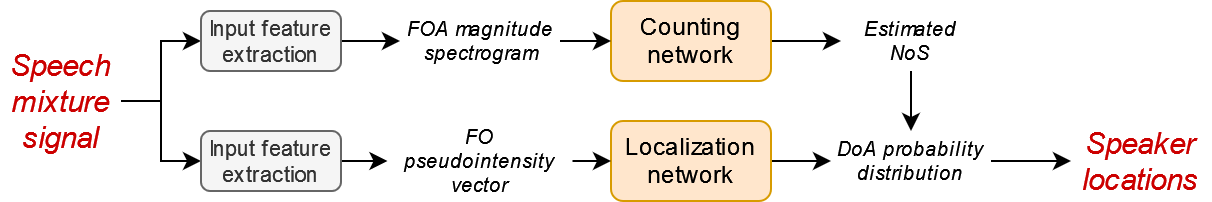
\includegraphics[width=1.\linewidth]{Images/chap8/nosEstimationPipeline.png}
    \end{adjustbox}
    \captionof{figure}[Processing pipeline of a localization system using the estimated NoS of a counting network]{Processing pipeline of an SSL system using the estimated NoS of a counting network.}
    \label{fig:nosEstimationPipeline}
\end{figure}

The processing pipeline of the proposed system is illustrated in Fig.~\ref{fig:nosEstimationPipeline}. An input speech mixture is first transformed into the input features of the counting and localization networks; that is, the FOA magnitude spectrograms and the FO-PIV, respectively. Then each network processes its respective input feature to generate the output: a NoS probability distribution from the counting network, and a DoA probability distribution from the localization network. The estimated NoS is first obtained as the class with the highest probability of the counting network output, as in Chapter \ref{chap:counting}. This estimated NoS then determines the number of peaks to extract from the localization network DoA distribution output. Note that for the evaluation of the system, the estimated DoAs are associated with the ground-truth labels using the Hungarian algorithm \cite{kuhn_hungarian_1955}, as already done in Section~\ref{ss:multiLocaClassif}.

\subsubsection{Counting and localization networks}

The counting network adopted in this experiment is the same as in Chapter~\ref{chap:counting}, with $T=20$ (number of frames in the input sequence) and $K=3$ (size of the convolution kernels), and using the optimal frame position as derived in Section~\ref{ss:accuracyAlongTheSequence} to maximize the counting accuracy. However, we retrain this network for a maximum number of sources $J=3$. The first reason for choosing this setting here is that we localize at most $3$ speakers simultaneously. We thus retrain the network to include the $3$-source constraint, as we conjecture that it would perform better than the $5$-source variant. The second reason is to provide a fair comparison of detection and counting metrics with the multi-task networks described in Section~\ref{sec:Multi-task-counting-loc} of this chapter.

For the localization network, we use Model $M_{5,2}$ detailed in Section~\ref{ss:multiLocalizationfeatureExtractionModule}.\footnote{We use here Model $M_{5,2}$ instead of $M_{6,4}$ as in Chapter~\ref{chap:multisourceLocalization} because the experiments on the feature extraction module were not concluded yet at the time of the study presented in the present chapter.} We recall that this model is composed a feature extraction module made of $5$ convolutional blocks, then 2 BiLSTM layers followed by 2 feedforward layers.

\subsection{Experimental protocol}
\subsubsection{Training and testing data}
\label{ss:trainingAndTestingNosPrediction}

As we consider here speaker counting in addition to localization, we employ a training dataset that is similar to the one described in Section~\ref{ss:countingTrainingData}. Both networks are trained using the same dataset. The generated signals are $15$-s long reverberant and noisy conversation-like mixtures, with a varying number of speakers. We limit the maximum number of speakers to $3$ (instead of $5$ in Chapter~\ref{chap:counting}) to be consistent with Chapter~\ref{chap:multisourceLocalization} on multi-speaker localization. Simulated SRIRs are used to create the mixtures, along with TIMIT \cite{garofolo_timit_1993} excerpts.

We evaluate our model on generated test sets that are similar to the ones described in Section~\ref{ss:countingTestingData} (\textit{i.e.}, with simulated SRIRs and real SRIRs, and up to $3$ simultaneous speakers).

\subsubsection{Baselines}

To assess the interest of using the estimated NoS provided by the counting network, we compare it with the use of the ground-truth NoS (referred as the \textit{oracle} method) and the NoS estimated using a thresholding method (we test several threshold values $\beta = 0.1, 0.2, 0.5$). To do that, we simply replace the estimated NoS from the counting network with the other considered NoS estimates.

\subsubsection{Metrics}
\label{ss:detectionCountingLocalizationMetrics}

To measure the performance of the proposed joint speaker counting and localization system, we calculate counting, detection and localization metrics. Regarding counting metrics, we compute the accuracy $A_{ij}$ and the mean absolute error $M_i$, as in Chapter~\ref{chap:counting}. We also consider the detection precision, which is defined as the percentage of estimated DoAs which correspond to actual DoAs, and the detection recall, which is as the percentage of actual DoAs that are estimated by the system. For the localization metrics, we consider only the true positives, \emph{i.e.}, the DoA estimations actually assigned to one label, and we calculate the localization accuracy (for angular error tolerance of $10$\textdegree~and $15$\textdegree) and the mean and median angular errors, as in Chapters~\ref{chap:tdvv} and \ref{chap:multisourceLocalization}.

\subsection{Results}
\label{ss:hybridNosPredictionResults}

\begin{table}[t]
    \begin{adjustbox}{width=1.1\textwidth,center}
    \begin{tabular}{|c|cccc|cccc|}
        \hline
        \multirow{3}{*}{\textbf{Counting method}} & \multicolumn{4}{c|}{\textbf{Simulated SRIRs}}                                                                                                                   & \multicolumn{4}{c|}{\textbf{Real SRIRs}}                                                                                                                        \\ \cline{2-9} 
                                                  & \multicolumn{2}{c}{\textbf{Detection}}                                & \multicolumn{2}{c|}{\textbf{Counting}}                                                  & \multicolumn{2}{c}{\textbf{Detection}}                                & \multicolumn{2}{c|}{\textbf{Counting}}                                                 \\
                                                  & \multicolumn{1}{l}{\textbf{Prec.}} & \multicolumn{1}{l}{\textbf{Rec.}} & \multicolumn{1}{l}{\textbf{Acc. (\%)}} & \multicolumn{1}{l|}{\textbf{Mean abs. error}} & \multicolumn{1}{l}{\textbf{Prec.}} & \multicolumn{1}{l}{\textbf{Rec.}} & \multicolumn{1}{l}{\textbf{Acc. (\%)}} & \multicolumn{1}{l|}{\textbf{Mean abs. error}} \\ \hline
        \textbf{Network}                          & 0.96                               & \textbf{0.92}                     & \textbf{82.5}                          & \textbf{0.2}                                  & 0.96                               & \textbf{0.82}                     & 70.3                                   & \textbf{0.3}                                  \\
        \textbf{Thres. ($\beta = 0.1$)}           & 0.96                               & 0.83                              & 74.1                                   & 0.3                                           & 0.95                               & 0.81                              & \textbf{70.6}                          & \textbf{0.3}                                  \\
        \textbf{Thres. ($\beta = 0.2$)}           & 0.98                               & 0.75                              & 68.2                                   & 0.4                                           & 0.97                               & 0.71                              & 64.3                                   & 0.5                                           \\
        \textbf{Thres. ($\beta = 0.5$)}           & \textbf{0.99}                      & 0.55                              & 55.1                                   & 0.7                                           & \textbf{0.99}                      & 0.47                              & 47.9                                   & 0.8                                           \\ \hline
    \end{tabular}
    \end{adjustbox}
    \captionof{table}[Detection and counting results of the counting network and the thresholding methods on test datasets]{Detection and counting results of the counting network and the thresholding methods on test datasets with simulated and real SRIRs. Best results are in bold.}
    \label{tab:hybrid_nosInjectionCountingResults}
\end{table}

\begin{figure}[t]
    \centering
    \subfloat[Simulated SRIRs]{
        \begin{adjustbox}{width=1.3\textwidth,center}
            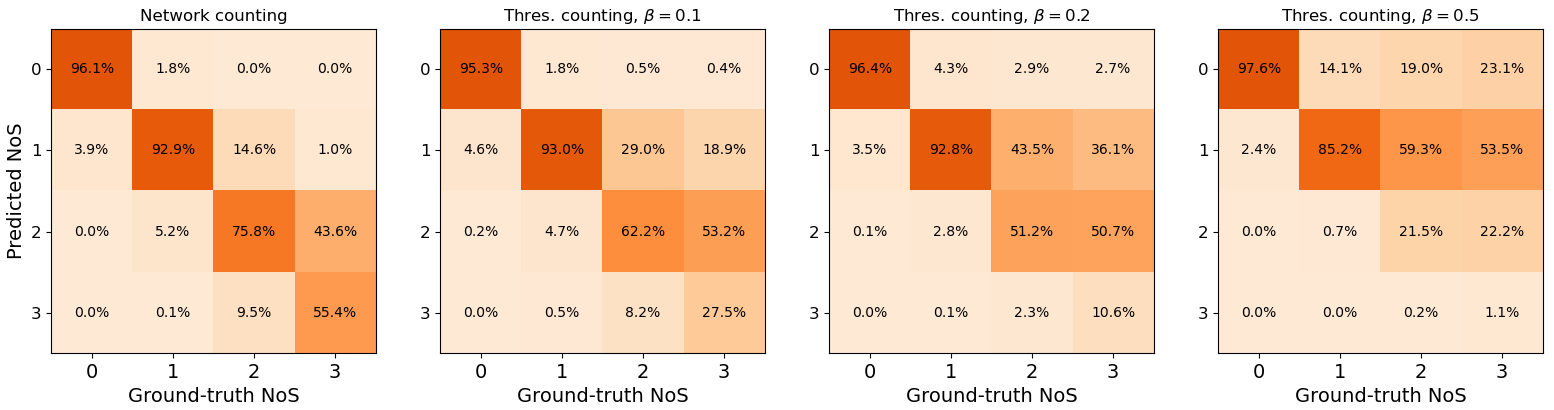
\includegraphics[width=1.\textwidth]{Images/chap8/hybrid_nosPrediction_confusionMatrix_simSrirs.png}
        \end{adjustbox}
    }\\
    \subfloat[Real SRIRs]{
        \begin{adjustbox}{width=1.3\textwidth,center}
            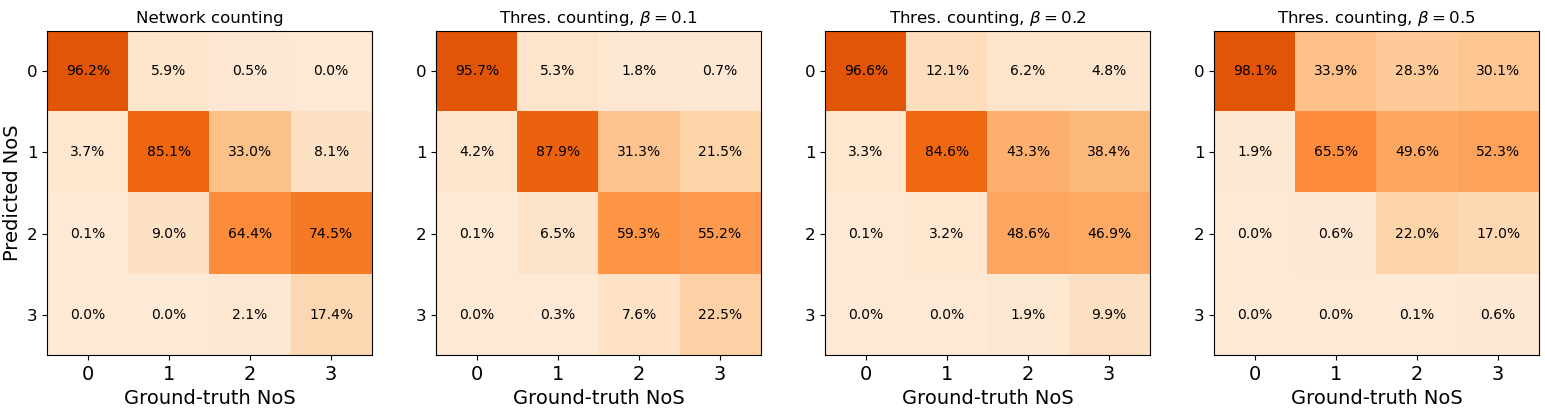
\includegraphics[width=1.\textwidth]{Images/chap8/hybrid_nosPrediction_confusionMatrix_realSrirs.png}
        \end{adjustbox}
    }
    \captionof{figure}[Confusion matrices of the accuracy $A_{ij}$ for several counting methods]{Confusion matrices of the accuracy $A_{ij}$ for several counting methods: a neural network counting method and a thresholding method for several values of the threshold $\beta$.}
    \label{fig:hybrid_nosPrediction_confusionMatrices}
\end{figure}

\begin{figure}[t]
    \centering
    \subfloat[Simulated SRIRs]{
        \begin{adjustbox}{width=1.2\textwidth,center}
            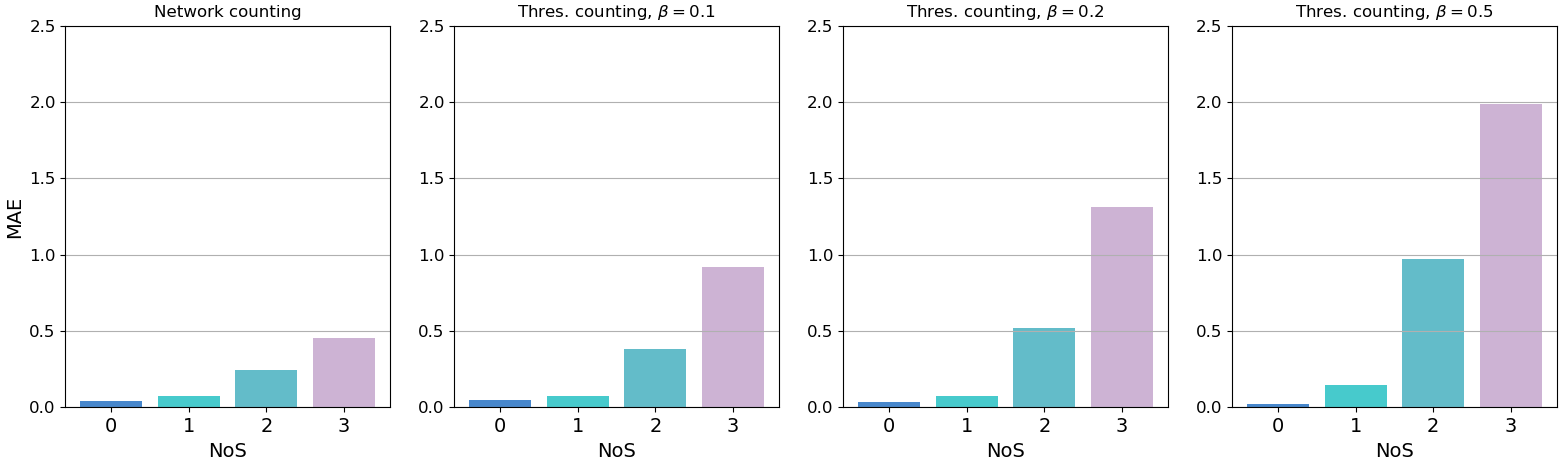
\includegraphics[width=1.\textwidth]{Images/chap8/hybrid_nosPrediction_mae_simSrirs.png}
        \end{adjustbox}
    }\\
    \subfloat[Real SRIRs]{
        \begin{adjustbox}{width=1.2\textwidth,center}
            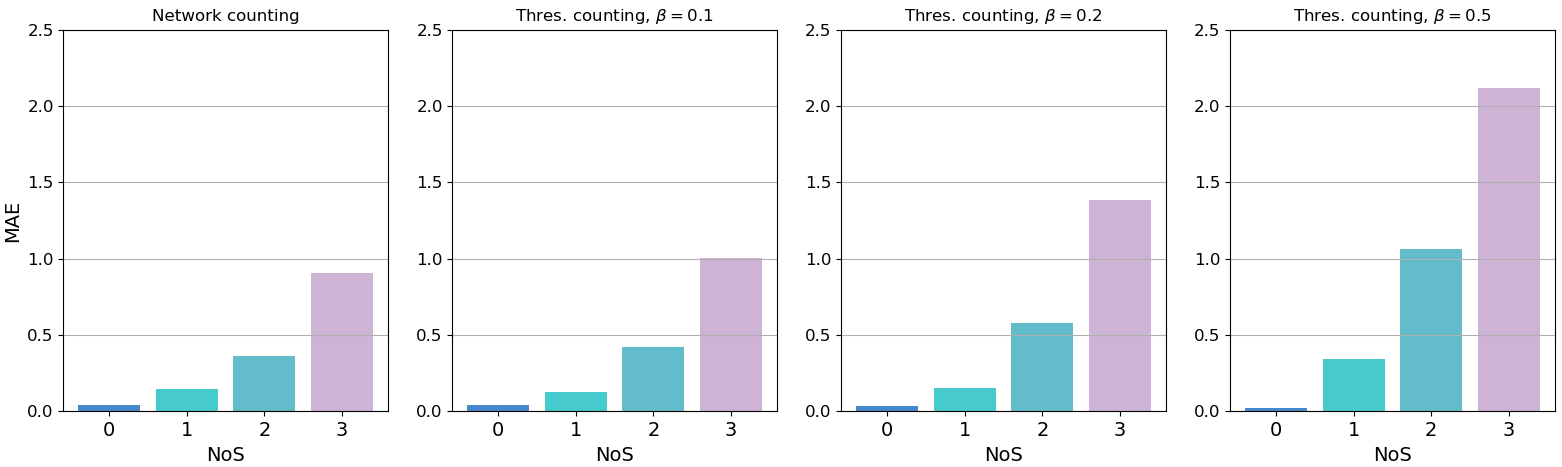
\includegraphics[width=1.\textwidth]{Images/chap8/hybrid_nosPrediction_mae_realSrirs.png}
        \end{adjustbox}
    }
    \captionof{figure}[Mean absolute errors $M_i$ for several counting methods]{Mean absolute errors $M_i$ for several counting methods: a neural network counting method and a thresholding method for several values of the threshold $\beta$.}
    \label{fig:hybrid_nosPrediction_mae}
\end{figure}

\begin{figure}[t]
    \centering
    \begin{adjustbox}{width=1.1\textwidth,center}
        \subfloat[Simulated SRIRs]{
        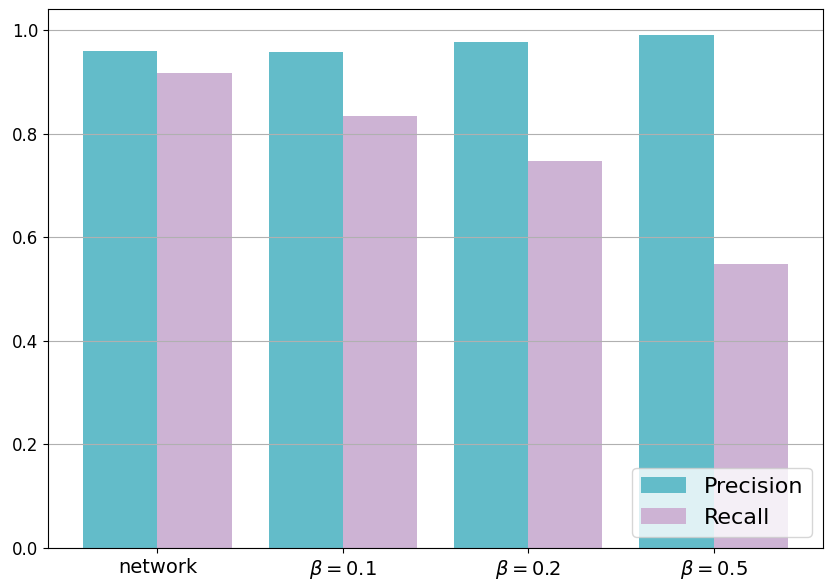
\includegraphics[width=.45\textwidth]{Images/chap8/hybrid_nosPrediction_detection_simSrirs.png}
        }
        \subfloat[Real SRIRs]{
            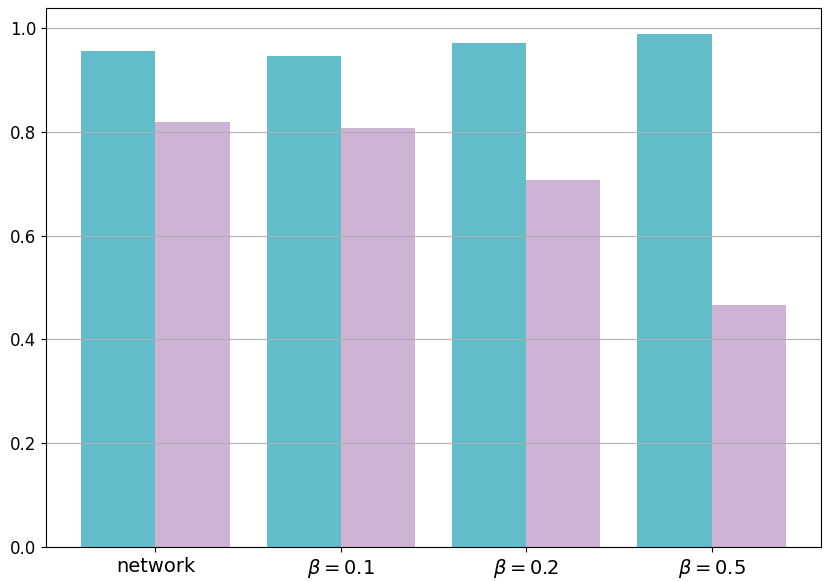
\includegraphics[width=.45\textwidth]{Images/chap8/hybrid_nosPrediction_detection_realSrirs.png}
        }
    \end{adjustbox}
    \captionof{figure}[Detection precision and recall for several counting methods]{Detection precision and recall for several counting methods: a neural network counting method and a thresholding method for several thresholds $\beta$.}
    \label{fig:hybrid_nosPrediction_prediction}
\end{figure}

\begin{table}[t]
\begin{adjustbox}{width=1.1\textwidth,center}
    \begin{tabular}{|c|cccc|cccc|}
    \hline
    \multirow{3}{*}{\textbf{Counting method}} & \multicolumn{4}{c|}{\textbf{Simulated SRIRs}}                                                     & \multicolumn{4}{c|}{\textbf{Real SRIRs}}                                                          \\ \hline
                                              & \multicolumn{2}{c}{\textbf{Accuracy (\%)}}      & \multicolumn{2}{c|}{\textbf{Angular error (°)}} & \multicolumn{2}{c}{\textbf{Accuracy (\%)}}      & \multicolumn{2}{c|}{\textbf{Angular error (°)}} \\
                                              & \textbf{\textless 10°} & \textbf{\textless 15°} & \textbf{Mean}         & \textbf{Median}        & \textbf{\textless 10°} & \textbf{\textless 15°} & \textbf{Mean}         & \textbf{Median}        \\ \hline
    Oracle                           & 75.2                   & 81.5                   & 15.5                  & 5.2                    & 56.2                   & 72.9                   & 18.3                  & 9.3                    \\
    Neural network                   & 78.7                   & 84.8                   & 12.9                  & 5.1                    & 62.8                   & 81.1                   & 13.2                  & 8.8                    \\
    Threshold ($\beta=0.1$)          & 86.2                   & 92.1                   & 8.4                   & 4.5                    & 66.2                   & 85.2                   & 10.5                  & 8.4                    \\
    Threshold ($\beta=0.2$)          & 88.9                   & 94.0                   & 7.4                   & 4.2                    & 68.6                   & 87.3                   & 10.0                  & 8.2                    \\
    Threshold ($\beta=0.5$)          & \textbf{93.3}                   & \textbf{96.4}                   & \textbf{6.0}                   & \textbf{3.9}                    & \textbf{72.9}                   & \textbf{90.0}                   & \textbf{9.2}                   & \textbf{7.9}                   \\ \hline
    \end{tabular}
\end{adjustbox}
\captionof{table}[Localization accuracy and angular errors for several counting methods]{Localization accuracy and angular errors for several counting methods. Best results are in bold.}
\label{tab:hybrid_nosPrediction_localization}
\end{table}

The counting metrics are showed in Table~\ref{tab:hybrid_nosInjectionCountingResults} and displayed in Fig.~\ref{fig:hybrid_nosPrediction_confusionMatrices} and \ref{fig:hybrid_nosPrediction_mae} as confusion matrices and $M_i$ bar charts, respectively. The prediction precision and recall are shown in  Fig.~\ref{fig:hybrid_nosPrediction_prediction}. Note that these metrics are not provided for the oracle method since they are all maximal. Table~\ref{tab:hybrid_nosPrediction_localization} presents the localization results (again, only for correctly detected sources).

When we look at the counting metrics, we can see the benefit of using a neural-based counting system over the traditional thresholding method. In the detection and counting results of Table~\ref{tab:hybrid_nosInjectionCountingResults}, we can first observe the quite high performance of the counting network on the dataset with simulated SRIRs, with at least $0.90$ of detection precision and recall and a mean absolute error of $0.2$ only. On the dataset with real SRIRs, the results are less favorable, especially regarding the detection recall with reaches $0.82$ and the counting accuracy which is $70.3$\%, emphasizing that in real conditions the counting network sometimes underestimates the NoS, thus missing to localize occasional speakers.
Regarding the detailed counting metrics in Fig.~\ref{fig:hybrid_nosPrediction_confusionMatrices} while the accuracy for classifying no-speech frames is almost perfect for all counting methods (\emph{i.e.}, with more than $95$\% accuracy), for speech frames the counting network clearly allows for a better speaker counting performance. On the dataset with simulated SRIRs, $75.8$\% of the $2$-speaker frames are correctly classified by the counting network where using a thresholding method leads to an accuracy of about $62$\%; for $3$-speaker frames, the accuracy reaches more than $55$\% for the neural network against only $27.5$\% using a threshold. We observe the same tendencies on the dataset with real SRIRs, except that the thresholding method with $\beta=0.1$ is slightly more accurate than the neural-based system for $1$- and $3$-speaker mixtures. The mean absolute error $M_i$ for every NoS is always lower for the network model than for the other methods. For instance, the $M_i$ for the counting network are lower than $0.5$ on signals with simulated SRIRs, meaning that the error committed by the network quite never exceeds 1 source (confirmed by the confusion matrices). Thresholding methods are less precise, especially when facing numerous simultaneous sources: for instance, $M_3$ for $\beta=1$ almost reaches $1$. On signals with real SRIRs, the mean absolute error for the thresholding method with $\beta$ is closer to that of the neural network, but it is still slightly higher. A reason why the thresholding method leads to close performance to the network's one could be because the localization network (on the output of which the thresholding method is applied) is more robust on signals with real SRIRs than the counting network.

The detection metrics in Fig.~\ref{fig:hybrid_multitask_prediction} confirm the advantage of using a neural network for speaker counting over a thresholding method. The detection recall of the network on both test datasets clearly surpasses that of all thresholding methods, while the precisions are about the same. By using a counting network, we miss only $10$\% and $20$\% of the sources, for the datasets with simulated and real SRIRs, respectively, while for the thresholding methods almost $20$\% of the sources are missed on signals with simulated SRIRs for $\beta=0.1$, and we even miss more than half of the speakers for real SRIRs when $\beta=0.5$. This highlights the fact that the thresholding methods often fail to detect some sources due to occasional too small peaks in the localization network output, even if the consecutive precision is almost perfect.

Finally, let us take a look at the localization metrics in Table~\ref{tab:hybrid_multitask_results} and Fig.~\ref{fig:hybrid_boxplots_multitask} while recalling that they are calculated by taking into account only the true positives. The thresholding method with the highest threshold value leads to the best localization metrics, but this is obtained at the cost of not detecting a lot of sources that are more difficult to localize, as shown by the detection results. On the contrary, we see that using the counting network allows to correctly detect sources that are not well localized, which leads to a two-digit mean angular error, whereas it remains under $10$\textdegree~with thresholding methods. The localization results with the counting network are relatively close to those using the ground-truth NoS, which are, by definition, optimal with respect to the source detection.

To conclude this study, the results show that using our speaker counting neural network allows to relax the strong assumption of knowing the NoS in advance. This counting network provides fairly accurate NoS estimations that can be used to localize speakers. This method has shown better detection performance over a thresholding method, which often leads to missing sources. Moreover, it can be observed that the localization performance using a speaker counting network closely approaches the one using the ground-truth NoS.

%-----------------------------------------------
%  NoS injection in a localization neural network
%-----------------------------------------------
\section{NoS injection in a localization neural network}
\label{sec:nosInjection}
\subsection{Method}
\label{ss:nosInjectionMethod}

In this section, we present a series of experiments in which we attempt to improve the localization network by injecting the NoS as an additional input information. The goal is to provide the network with an additional information hoping that it can improve the localization performance, with the intuition that it could help the network to output a cleaner DoA peak distribution. 

The proposed localization system with NoS injection is illustrated in Fig.~\ref{fig:nosInjectionPipeline}. The NoS is injected as an input feature into the localization network, in addition to the FO-PIV features. At this stage, we name it the \textit{injection NoS}. The NoS is also used further for peak-picking on the localization network output. We refer to this second use of the NoS as the \textit{prediction NoS}. The need for a distinction between the injection NoS and the prediction NoS will be made clear in the following.

\begin{figure}[t]
    \begin{adjustbox}{width=1.2\textwidth,center}
        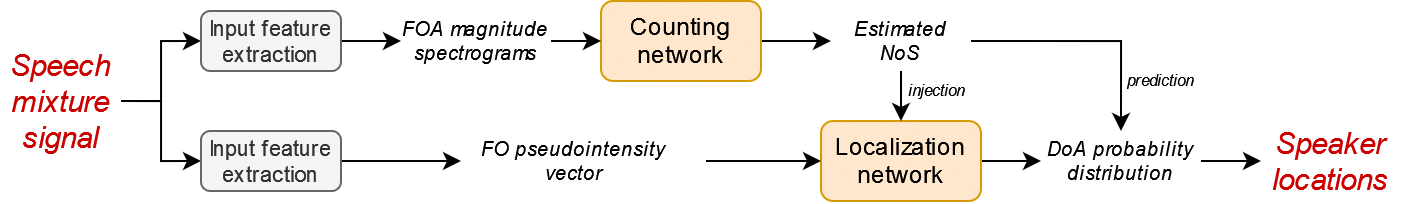
\includegraphics[width=1.\linewidth]{Images/chap8/nosInjectionPipeline.png}
    \end{adjustbox}
    \captionof{figure}[Processing pipeline of a localization system with NoS injection]{Processing pipeline of a localization system with NoS injection.}
    \label{fig:nosInjectionPipeline}
\end{figure}

We propose and test different ways to inject the NoS into the localization network, as illustrated in Fig.~\ref{fig:nosInjectionInLocalizationNetwork} and commented below. As in Section~\ref{sec:nosEstimation}, we opt for base model $M_{5,2}$ as proposed in Section~\ref{ss:multiLocalizationfeatureExtractionModule}. Note that, unlike in Chapter~\ref{chap:tdvv} and \ref{chap:multisourceLocalization}, here we do not average the DoA distribution over all frames of a sequence in the network output. Instead, we go back to a frame-wise prediction to demonstrate the usefulness of the counting DNN at high temporal resolution. Throughout several experiments, we try injecting the NoS in several positions in the neural network:
\begin{itemize}
    \item alongside the input features;
    \item after the feature extraction (and reshape) module;
    \item after the temporal analysis module;
    \item both after the feature extraction module and after the temporal analysis module;
    \item after the first feedforward layer.
\end{itemize}

\begin{figure}[t]
    \begin{adjustbox}{width=0.75\textwidth,center}
        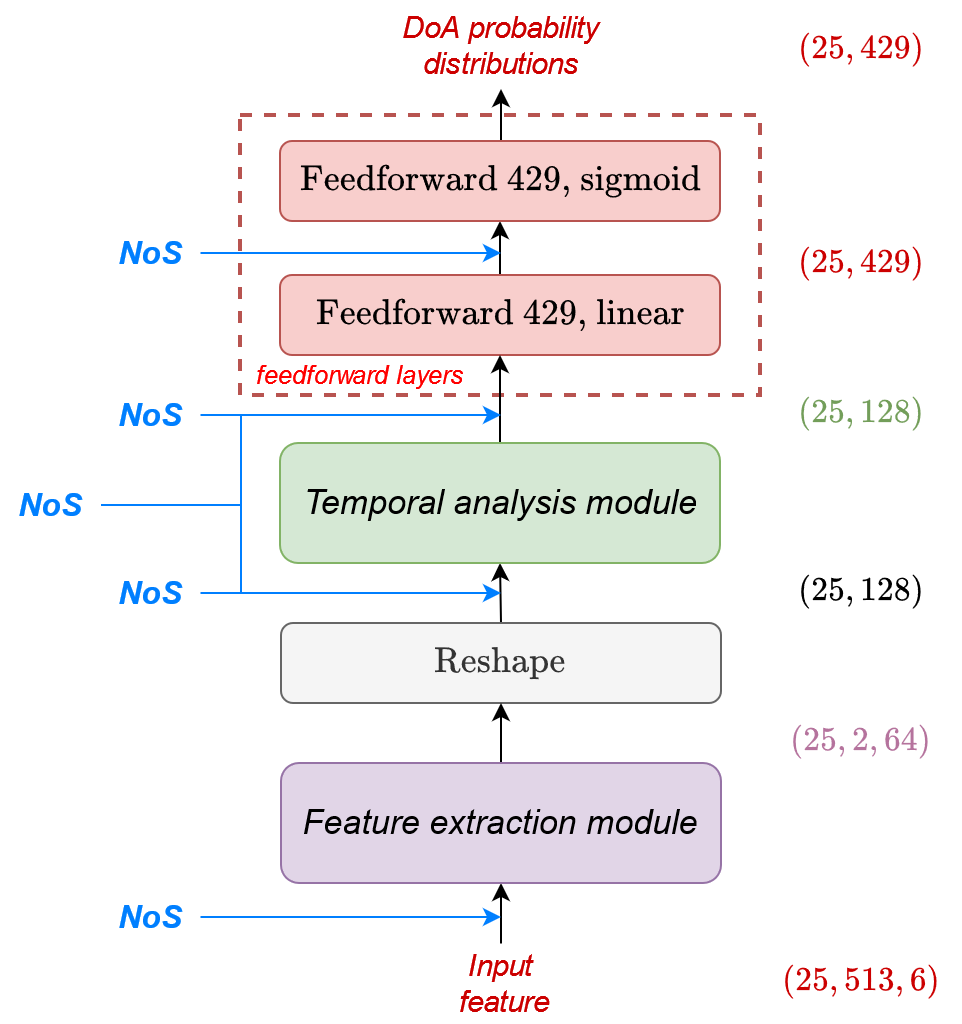
\includegraphics[width=1.\linewidth]{Images/chap8/nosInjectionNetwork.png}
    \end{adjustbox}
    \captionof{figure}[Tested positions for the NoS injection in the localization network]{Tested positions for the NoS injection in the localization network.}
    \label{fig:nosInjectionInLocalizationNetwork}
\end{figure}

The injection is done by concatenating the NoS feature with the feature tensor present at the place of injection. For each frame $t$, the NoS feature corresponding to the instantaneous NoS $J(t)$ is represented as a one-hot encoded vector $\mathbf{z}(t)$ of size $J+1$ where $J$ is the maximum number of speakers considered in the mixtures. This vector encodes the NoS information by setting $z_i(t) = 1$ if $i = J(t)$ and $z_i(t) = 0$ otherwise. The injection is done for each frame in the considered tensor, which is possible since the temporal dimension is preserved through all layers. The concatenation is carried out on the second dimension (akin to the input frequency dimension) for all frames. For instance, if the injection is done alongside the input feature of shape $(25, 513, 6)$, the tensor obtained after the concatenation is of shape $(25, 513+J+1, 6)$; if the injection is performed after the temporal analysis module, the new tensor shape is $(25, 128+J+1)$.

The different options for the injection position are motivated by different intuitions. Mixing the NoS feature with the FO-PIV feature seems strange since the convolutional layers will treat all this data at once, but this practice has proved to be beneficial in another audio task \cite{vogl_drum_2017}. Concatenating the NoS to the extracted feature after the convolutional layers seems a bit more reasonable since it can accompany the data modelled by the feature extraction module to help during the temporal analysis process, as the instantaneous NoS can vary in each frame. In the same vein, injecting the NoS feature just after the BiLSTM layers gives an additional cue for the network classification task performed by the two feedforward layers. We also tried adding the NoS feature just before the output, again with the idea of providing such an information alongside higher-level features. Injecting the NoS both before and after the temporal analysis module has been experimented afterwards based on the obtained results, as detailed below.

\subsection{Experimental protocol}
\subsubsection{Training and testing data}

To train these neural networks, we used the same training and testing datasets as in Section~\ref{sec:nosEstimation} (\emph{i.e.}, obtained by generating $15$-s long reverberant and noisy speech mixtures, with an instantaneous NoS varying from $0$ to $3$). Simulated SRIRs are used to generate the training signals, while for testing, we used the datasets of both simulated and recorded SRIRs.

During training, we use the ground-truth NoS both as the injection NoS and the prediction NoS. However, during inference in a practical use-case, we use the estimated NoS from the speaker counting network both for injection and prediction. In that manner, we train the network in an optimal way hoping that it will be robust enough when an imperfect NoS information is provided.

\subsubsection{Baselines}

To assess the benefit of NoS injection, we compare the proposed model with the base model $M_{5,2}$ (see Section~\ref{ss:multiLocalizationfeatureExtractionModule} for more details) without injection. Moreover, to gauge the robustness of such a network in real conditions, \emph{i.e.}, when the ground-truth NoS is not available, we evaluate the networks on the test datasets for different versions of the injection NoS and the prediction NoS independently:
\begin{itemize}
    \item The injection and prediction NoS are both the ground-truth NoS. This allows us to directly compare our proposed system with the oracle condition.
    \item The injection NoS is the ground-truth NoS and the prediction NoS is estimated by the speaker counting network. We evaluate the robustness of using an estimated NoS for the DoA prediction while the NoS input data is the ground-truth.
    \item The injection NoS is estimated by the neural network, and the prediction NoS is the ground-truth NoS. This last configuration allows to assess the network capacity to cope with the injection of an imperfect NoS, while being in an optimal condition for peak picking. 
\end{itemize}

In the following, using the ground-truth NoS for injection or for DoA peak-peaking is referred to as \textit{oracle} injection NoS and \textit{oracle} prediction NoS, respectively. Using the NoS provided by the counting neural network is referred to as \textit{estimated} injection NoS and \textit{estimated} prediction NoS.

\subsubsection{Metrics}

We use the same metrics as in Section~\ref{sec:nosEstimation}. In this series of experiments, we either use the ground-truth NoS, which leads perfect counting and detection scores, or the estimated NoS using the counting network, whose performance have been shown in Table~\ref{tab:hybrid_nosInjectionCountingResults} and discussed in Section~\ref{sec:nosEstimation}. Besides, we show the localization results which are the main interest in these experiments.

\subsection{Results}
\label{ss:hybridNosInjectionResults}

\begin{table}[t]
\centering
    \subfloat[Oracle injection NoS, oracle prediction NoS]{
        \begin{adjustbox}{width=1.2\textwidth,center}
            \begin{tabular}{|c|cccc|cccc|}
                \hline
                \multirow{3}{*}{\textbf{Injection position}}            & \multicolumn{4}{c|}{\textbf{Simulated SRIRs}}                                                    & \multicolumn{4}{c|}{\textbf{Real SRIRs}}                                                          \\ \cline{2-9} 
                                                                        & \multicolumn{2}{c}{\textbf{Accuracy (\%)}}     & \multicolumn{2}{c|}{\textbf{Angular error (°)}} & \multicolumn{2}{c}{\textbf{Accuracy (\%)}}     & \multicolumn{2}{c|}{\textbf{Angular error (°)}} \\
                                                                        & \textbf{\textless 10°} & \textbf{\textless 15°} & \textbf{Mean}         & \textbf{Median}        & \textbf{\textless 10°} & \textbf{\textless 15°} & \textbf{Mean}         & \textbf{Median}         \\ \hline
                No injection                                   & 75.2                   & 81.5                   & 15.5                  & 5.2                    & 56.2                   & 72.9                   & 18.3                  & 9.3                     \\
                Input                                          & 75.9                   & 81.9                   & 15.7                  & 5.1                    & 52.7                   & 70.4                   & 19.8                  & 9.5                     \\
                After feature extraction                       & 78.4                   & 83.3                   & 14.7                  & \textbf{4.8}           & 56.0                   & 73.4                   & 17.3                  & 9.2                     \\
                After temporal analysis                        & \textbf{80.1}          & \textbf{84.4}          & \textbf{13.7}         & \textbf{4.8}           & 53.9                   & 73.3                   & 18.2                  & 9.6                     \\
                After feature extrac. \& temp. analysis & 78.4                   & 83.4                   & 14.2                  & \textbf{4.8}           & \textbf{57.9}          & \textbf{74.3}          & \textbf{16.9}         & \textbf{9.0}            \\
                After feedforward layer                        & 76.1                   & 82.3                   & 14.9                  & 5.2                    & 55.5                   & 71.4                   & 19.7                  & 9.1                     \\ \hline
            \end{tabular}
            \label{tab:hybrid_nosInjection_oracleInj_oraclePred}
        \end{adjustbox}
    }

    \subfloat[Estimated injection NoS, oracle prediction NoS]{
        \begin{adjustbox}{width=1.2\textwidth,center}
            \begin{tabular}{|c|cccc|cccc|}
                \hline
                \multirow{3}{*}{\textbf{Injection position}}            & \multicolumn{4}{c|}{\textbf{Simulated SRIRs}}                                                    & \multicolumn{4}{c|}{\textbf{Real SRIRs}}                                                          \\ \cline{2-9} 
                                                                        & \multicolumn{2}{c}{\textbf{Accuracy (\%)}}     & \multicolumn{2}{c|}{\textbf{Angular error (°)}} & \multicolumn{2}{c}{\textbf{Accuracy (\%)}}     & \multicolumn{2}{c|}{\textbf{Angular error (°)}} \\
                                                                        & \textbf{\textless 10°} & \textbf{\textless 15°} & \textbf{Mean}         & \textbf{Median}        & \textbf{\textless 10°} & \textbf{\textless 15°} & \textbf{Mean}         & \textbf{Median}         \\ \hline
                No injection                                   & 75.2                   & 81.5                   & 15.5                  & 5.2                    & 56.2                   & \textbf{72.9}          & \textbf{18.3}         & 9.3                     \\
                Input                                         & 75.5                   & 81.6                   & 16.1                  & 5.2                    & 51.4                   & 69.0                   & 20.7                  & 9.6                     \\
                After feature extraction                       & 77.6                   & 82.2                   & 15.4                  & \textbf{4.8}           & 54.9                   & 71.4                   & 18.9                  & 9.3                     \\
                After temporal analysis                        & \textbf{79.5}          & \textbf{83.9}          & \textbf{14.2}         & \textbf{4.8}           & 52.7                   & 71.9                   & 19.5                  & 9.6                     \\
                After feature extrac. \& temp. analysis & 77.5                   & 82.2                   & 15.1                  & 5.0                    & \textbf{56.8}          & 72.5                   & 19.0                  & \textbf{9.1}            \\
                After feedforward layer                        & 76.1                   & 82.6                   & 14.9                  & 5.2                    & 55.4                   & 71.3                   & 19.8                  & 9.2                     \\ \hline
            \end{tabular}
            \label{tab:hybrid_nosInjection_estimateInj_oraclePred}
        \end{adjustbox}
    }
        
    \subfloat[Oracle injection NoS, estimated prediction NoS]{
        \begin{adjustbox}{width=1.2\textwidth,center}
            \begin{tabular}{|c|cccc|cccc|}
                \hline
                \multirow{3}{*}{\textbf{Injection position}}            & \multicolumn{4}{c|}{\textbf{Simulated SRIRs}}                                                    & \multicolumn{4}{c|}{\textbf{Real SRIRs}}                                                          \\ \cline{2-9} 
                                                                        & \multicolumn{2}{c}{\textbf{Accuracy (\%)}}     & \multicolumn{2}{c|}{\textbf{Angular error (°)}} & \multicolumn{2}{c}{\textbf{Accuracy (\%)}}     & \multicolumn{2}{c|}{\textbf{Angular error (°)}} \\
                                                                        & \textbf{\textless 10°} & \textbf{\textless 15°} & \textbf{Mean}         & \textbf{Median}        & \textbf{\textless 10°} & \textbf{\textless 15°} & \textbf{Mean}         & \textbf{Median}         \\ \hline
                No injection                                   & 78.7                   & 84.8                   & 12.9                  & 5.1                    & 62.8                   & 81.1                   & 13.2                  & 8.8                     \\
                Input                                          & 79.6                   & 85.4                   & 13.3                  & 4.8                    & 59.0                   & 78.4                   & 14.8                  & 8.6                     \\
                After feature extraction                       & 81.9                   & 86.5                   & 12.4                  & 4.6                    & 61.5                   & 80.7                   & \textbf{12.7}         & 8.5                     \\
                After temporal analysis                        & \textbf{83.8}          & \textbf{87.8}          & \textbf{11.5}         & \textbf{4.5}           & 60.1                   & 81.1                   & 13.5                  & 9.0                     \\
                After feature extrac. \& temp. analysis & 82.3                   & 86.7                   & 11.9                  & 4.6                    & \textbf{63.9}          & \textbf{82.1}          & 12.8                  & \textbf{8.3}            \\
                After feedforward layer                        & 79.6                   & 85.9                   & 12.6                  & 4.8                    & 61.6                   & 79.4                   & 14.5                  & \textbf{8.3}            \\ \hline
            \end{tabular}
            \label{tab:hybrid_nosInjection_oracleInj_estimatePred}
        \end{adjustbox}
    }
        
    \subfloat[Estimated injection NoS, estimated prediction NoS]{
        \begin{adjustbox}{width=1.2\textwidth,center}
            \begin{tabular}{|c|cccc|cccc|}
                \hline
                \multirow{3}{*}{\textbf{Injection position}}            & \multicolumn{4}{c|}{\textbf{Simulated SRIRs}}                                                    & \multicolumn{4}{c|}{\textbf{Real SRIRs}}                                                          \\ \cline{2-9} 
                                                                        & \multicolumn{2}{c}{\textbf{Accuracy (\%)}}     & \multicolumn{2}{c|}{\textbf{Angular error (°)}} & \multicolumn{2}{c
                                                                        }{\textbf{Accuracy (\%)}}     & \multicolumn{2}{c|}{\textbf{Angular error (°)}} \\
                                                                        & \textbf{\textless 10°} & \textbf{\textless 15°} & \textbf{Mean}         & \textbf{Median}        & \textbf{\textless 10°} & \textbf{\textless 15°} & \textbf{Mean}         & \textbf{Median}         \\ \hline
                No injection                                   & 78.7                   & 84.8                   & 12.9                  & 5.1                    & 62.8                   & 81.1                   & 13.2                  & 8.8                     \\
                Input                                          & 79.5                   & 85.5                   & 13.3                  & 4.8                    & 59.0                   & 78.7                   & 14.6                  & 8.7                     \\
                After feature extraction                       & 82.0                   & 86.3                   & 12.4                  & 4.6                    & 62.3                   & 81.1                   & \textbf{12.6}         & 8.4                     \\
                After temporal analysis                        & \textbf{83.8}          & \textbf{87.7}          & \textbf{11.5}         & \textbf{4.5}           & 59.9                   & 81.1                   & 13.5                  & 9.0                     \\
                After feature extrac. \& temp. analysis & 82.3                   & 86.5                   & 12.1                  & 4.6                    & \textbf{64.4}          & \textbf{82.4}          & 12.7                  & \textbf{8.2}            \\
                After feedforward layer                        & 79.7                   & 86.0                   & 12.6                  & 4.8                    & 61.7                   & 79.4                   & 14.5                  & 8.3                     \\ \hline
            \end{tabular}
            \label{tab:hybrid_nosInjection_estimateInj_estimatePred}
        \end{adjustbox}
    }

    \captionof{table}[Accuracy and angular errors of the localization network with NoS injection]{Accuracy and angular errors of the localization network with NoS injection, for different injection positions and the four combinations of oracle/estimated NoS for injection and prediction. Best results are in bold.}
    \label{tab:hybrid_nosInjection}
\end{table}

Table~\ref{tab:hybrid_nosInjection} shows the localization results of the model with all considered injection positions, and for the four different combinations of oracle/estimated NoS and injection/prediction. 

First, let us clarify that the results when no injection is used are obtained with a peak-picking of the DoA output distribution based on the ground-truth NoS for Tables~\ref{tab:hybrid_nosInjection_oracleInj_oraclePred} and \ref{tab:hybrid_nosInjection_estimateInj_oraclePred}, and on the estimated NoS for Tables~\ref{tab:hybrid_nosInjection_oracleInj_estimatePred} and \ref{tab:hybrid_nosInjection_estimateInj_estimatePred}, for a fair comparison with the models with NoS injection. Globally, we observe that most results with NoS injection are better than without injection. In all four tables, we notice that some injection positions almost always lead to better results than the model without injection. Particularly, this is the case when the injection is done after the temporal analysis module only, and both after the feature extraction and the temporal analysis modules. To give some numbers, when the only estimated NoS is used (Table~\ref{tab:hybrid_nosInjection_estimateInj_estimatePred}), the localization accuracy ($<10$\textdegree) for simulated SRIRs is increased from $78.7$\% without injection to $83.8$\% with injection after the temporal analysis module, and the median angular error is decreased from $5.1$\textdegree~to $4.5$\textdegree. On real SRIRs, the gain in performance is less noticeable, with an accuracy increase of only $1.6$\% and a median error decrease of $0.6$\textdegree~when injecting the NoS both after the feature extraction and temporal analysis modules. We can hence conclude that estimated NoS injection actually helps the localization network to achieve a better performance.

If we look at Table~\ref{tab:hybrid_nosInjection_oracleInj_oraclePred}, where only the ground-truth NoS is used for injection and DoA extraction, which can be considered as the optimal configuration, we also observe a gain in performance when injecting the NoS in several positions, such as after the temporal analysis module or after the feature extraction module. This confirms the interest of NoS injection. Now, when looking at Table~\ref{tab:hybrid_nosInjection_estimateInj_oraclePred}, whose difference with Table~\ref{tab:hybrid_nosInjection_oracleInj_oraclePred} is that we inject an estimated (thus imperfect) NoS instead of the ground-truth NoS (but still using the oracle prediction NoS), we observe than the results are almost as good as in the fully optimal conditions of Table~\ref{tab:hybrid_nosInjection_oracleInj_oraclePred}. This suggests that the counting network provides an estimated NoS with high enough accuracy, so that the injection of the estimated NoS is beneficial for the localization network. The loss in accuracy is around $1$\% when using an estimated injection NoS, while the median angular error is almost unaffected.

Focusing on Table~\ref{tab:hybrid_nosInjection_oracleInj_estimatePred} for which the ground-truth NoS is injected and the estimated NoS is used for DoA peak picking, we observe the common raise in localization performance due to the miss detection of certain sources, which surely corresponds to the difficult cases, with a bad localization accuracy. This observation is identical when comparing the results model without injection between Tables~\ref{tab:hybrid_nosInjection_oracleInj_oraclePred}, \ref{tab:hybrid_nosInjection_estimateInj_oraclePred} and Tables~\ref{tab:hybrid_nosInjection_oracleInj_estimatePred}, \ref{tab:hybrid_nosInjection_estimateInj_estimatePred}. Then, as above, comparing Table~\ref{tab:hybrid_nosInjection_estimateInj_estimatePred} with Table~\ref{tab:hybrid_nosInjection_oracleInj_estimatePred} allows us to assess the use of an estimated NoS for the injection instead of the ground-truth NoS. Again, we can see that the results are almost the same, and are even closer than when comparing the numbers of Tables~\ref{tab:hybrid_nosInjection_oracleInj_oraclePred} and \ref{tab:hybrid_nosInjection_estimateInj_oraclePred}. This indicates that when an estimated NoS is used for DoA peak extraction, using the same estimated NoS for injection is almost as effective as using the ground-truth NoS. This also shows that the use of inexact (estimated) NoS is more detrimental for peak-picking, than it is when used for injection.

\begin{figure}[ht!]
    \centering
        \subfloat[Simulated SRIRs]{
            \begin{adjustbox}{width=1.1\textwidth,center}
                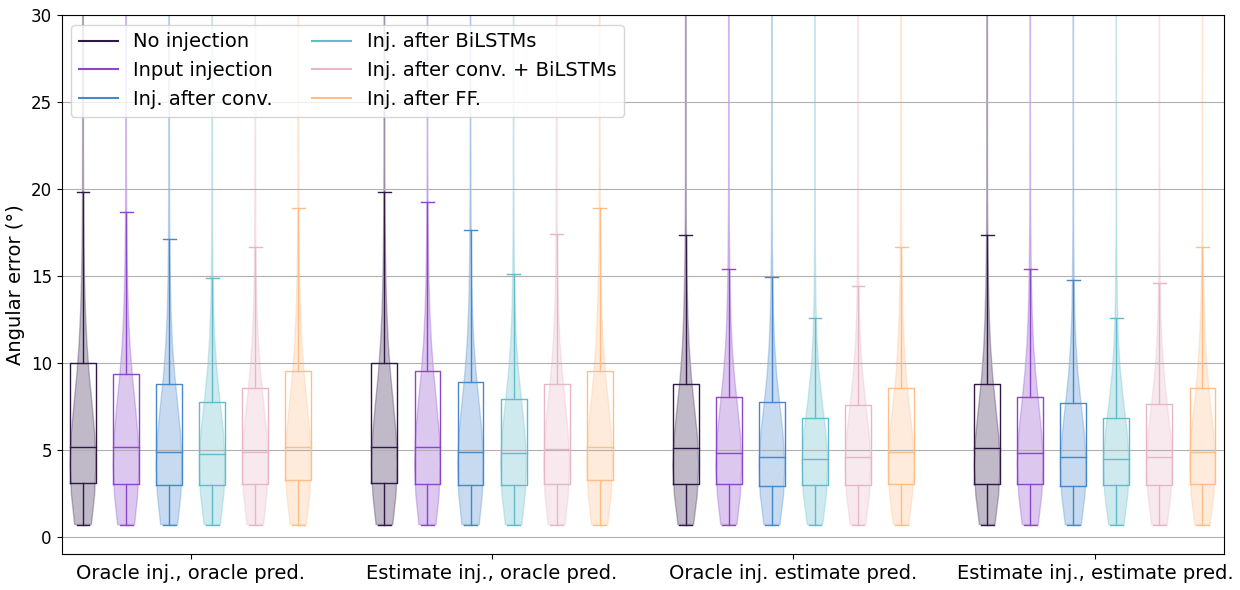
\includegraphics[width=.5\textwidth]{Images/chap8/hybrid_boxplots_nosInjection_simSRIRs.png}
            \end{adjustbox}
        }\\
        \subfloat[Real SRIRs]{
            \begin{adjustbox}{width=1.1\textwidth,center}
                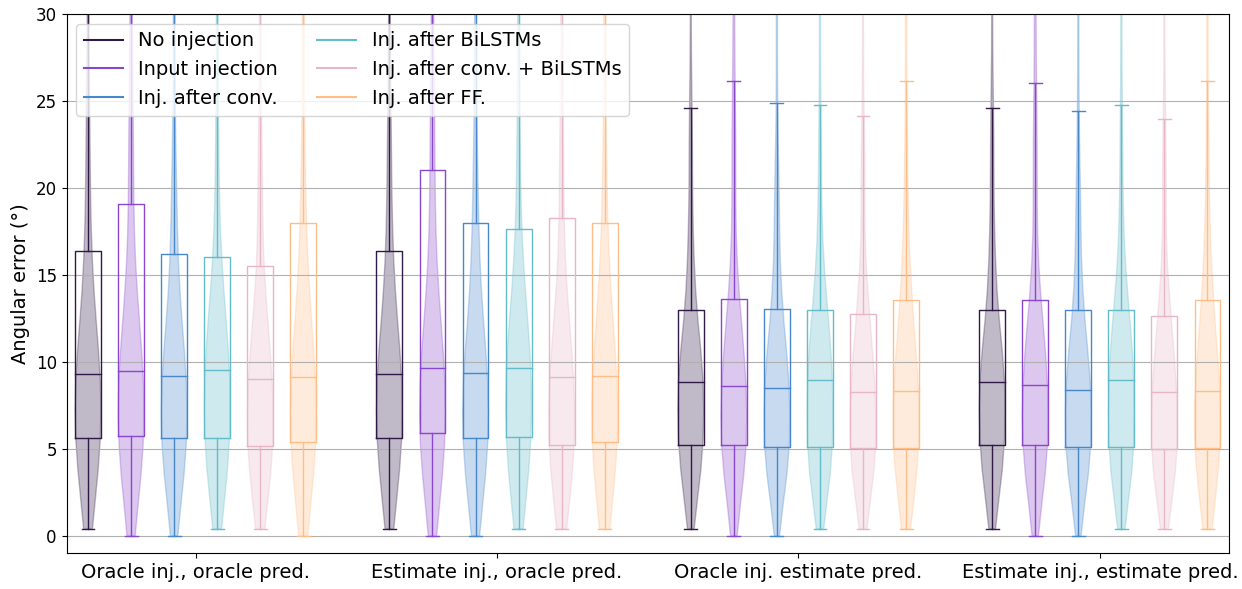
\includegraphics[width=.5\textwidth]{Images/chap8/hybrid_boxplots_nosInjection_realSRIRs.png}
            \end{adjustbox}
        }
    \captionof{figure}[Boxplots of the angular errors of the localization network for several injection positions]{Boxplots of the angular errors of the localization network for several injection positions, and considering several NoS derivation configurations.}
    \label{fig:hybrid_boxplots_nosInjection}
\end{figure}

Finally, the boxplots and violin plots in Fig.~\ref{fig:hybrid_boxplots_nosInjection} underline the interest of NoS injection on data with simulated SRIRs, however the results are less convincing on real-world data. On the dataset with simulated SRIRs, we clearly observe the advantage of NoS injection as it allows to reduce the angular error variance, although the median angular error almost remains unchanged. This figure confirms that the best injection location seems to be both after the feature extraction and temporal analysis modules. Regarding the dataset with real SRIRs, we notice that when the ground-truth NoS is used for DoA extraction, the injection leads a higher error variance, especially with an estimated NoS injection. With a DoA extraction based on an estimated NoS, the boxplots indicate that the injection results are on par with the model without injection.

To conclude this study, we observe a certain interest of injecting the NoS as an additional input feature into the localization network. While injecting it directly alongside the intensity-based input features, or just before the output layer, has not been beneficial, we notice than NoS injection after the feature extraction module, after the temporal analysis module or after both modules leads to a clear gain in localization performance on the dataset with simulated SRIRs. On the dataset with real SRIRs, the interest of injection is slightly more moderate but several figures confirm its usefulness. Throughout a careful analysis, we manage to show the robustness of relying on an estimated NoS instead of the ground-truth NoS at both the injection and the prediction levels.

%-----------------------------------------------
%  Multi-task speaker counting and localization network
%-----------------------------------------------
\clearpage
\section{Multi-task speaker counting and localization network}
\label{sec:Multi-task-counting-loc}

In this last series of experiments, we propose to consider a multi-task neural network scheme that directly estimates both the NoS and the speaker locations at the same time. Multiple designs are tested, inspired by the architectures of the speaker counting and localization networks.

\subsection{Method}

\subsubsection{Input feature}
\label{ss:multi-taskInputFeature}

In this new approach of the joint counting and localization system, we use as input features a combination of both input features employed in the previously presented separate counting and localization networks (\emph{i.e.}, the magnitude FOA spectrograms and the FO-PIV feature).

As explained in Section~\ref{ss:multi-taskNetworkArchitectures} below, in a first design of multi-task network, we combine both input features in the same input tensor. Using the same parameterization as before, the magnitude FOA spectrograms consists of a tensor of size $(25, 513, 4)$ and the normalized FO-PIV feature size is $(25, 513, 6)$. Therefore, the combined features at the input of the multi-task network are obtained by concatenating these two tensor features along the third dimension, leading to a new tensor of size $(25,513,10)$. Indeed, these features are of a very different nature, and simple concatenation may seem ad-hoc. However, we deem that the network is capable of learning how to extract the useful information from such an input.

We also designed a multi-task network in which the two input features are fed into two separate input branches, corresponding to two similar feature extraction modules (see Section~\ref{ss:multi-taskNetworkArchitectures}). In this system, these input features are obtained identically as in the separate counting and localization networks: normalization is employed across the whole training dataset for the magnitude spectrograms, and the normalized version of the FO-PIV is used.

\subsubsection{Multi-task network architectures}
\label{ss:multi-taskNetworkArchitectures}

During our experiments, we consider several multi-task network architectures, which are illustrated in Fig.~\ref{fig:hybrid_multi-taskNetworkArchitectures}.

\begin{figure}[t]
    \centering
    \begin{adjustbox}{width=1.3\textwidth,center}
        \subfloat[Architecture with combined input features]{
                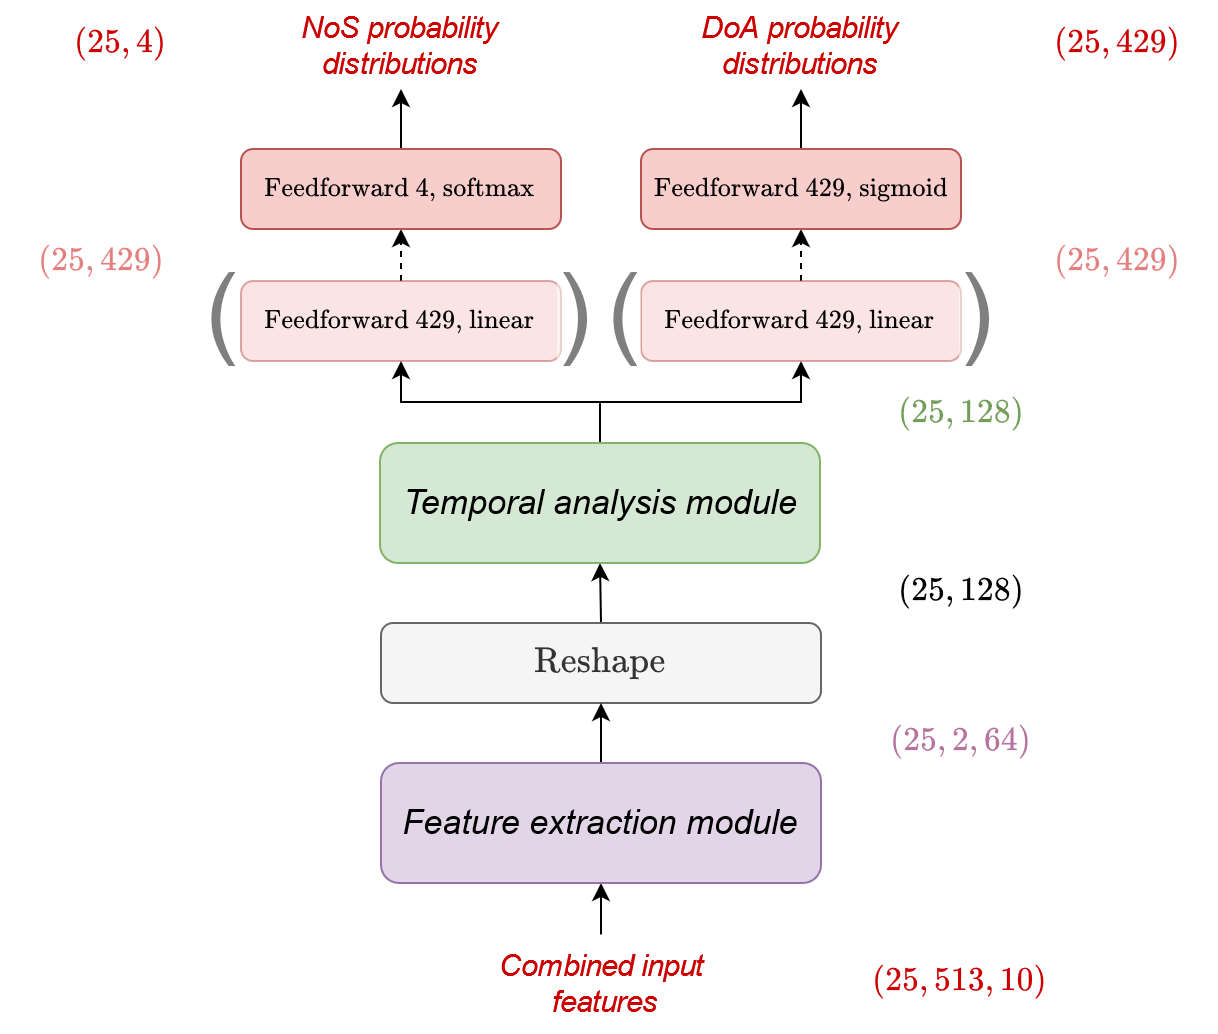
\includegraphics[width=.6\textwidth]{Images/chap8/multitaskNetwork_combinedInput.png}
        }
        \subfloat[Architecture with separated input features]{
                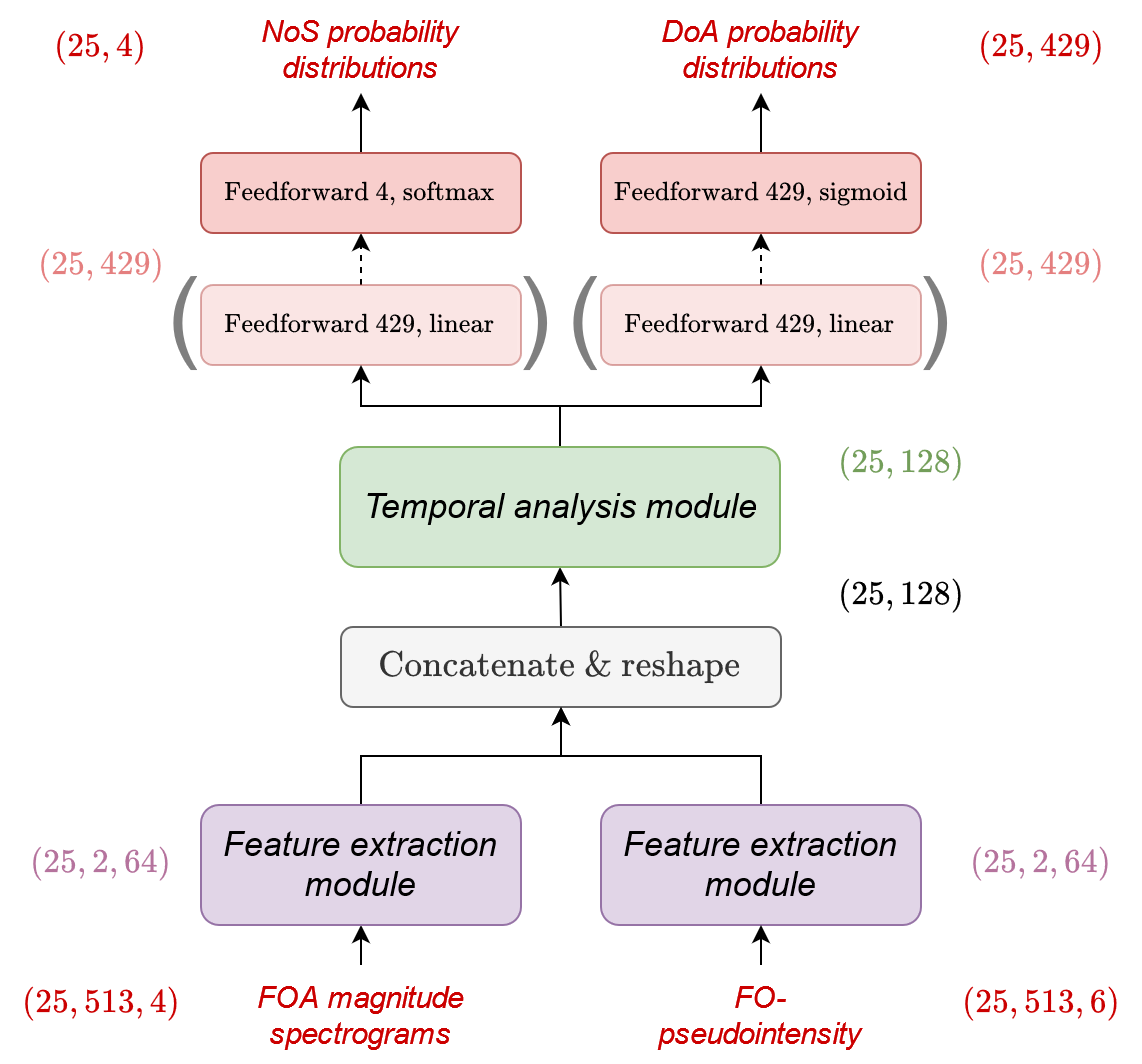
\includegraphics[width=.6\textwidth]{Images/chap8/multitaskNetwork_separateInput.png}
        }
    \end{adjustbox}
    \captionof{figure}[Architectures of the proposed multi-task counting and localization neural networks]{Architectures of the proposed multi-task counting and localization neural networks.}
    \label{fig:hybrid_multi-taskNetworkArchitectures}
\end{figure}

The first multi-task network we propose, shown in the left of  Fig.~\ref{fig:hybrid_multi-taskNetworkArchitectures}, is made of a common feature extraction module for both input features, which are concatenated into a single feature tensor as explained in Section~\ref{ss:multi-taskInputFeature} above. The overall architecture is still based on the model $M_{5,2}$ presented in Section~\ref{ss:multiLocalizationfeatureExtractionModule}, except for the feedforward layers. After the temporal analysis module, the output tensor is fed into two distinct branches, one for the counting task and the other for the localization task. Each branch contains the same number of feedforward layers $D$, which is a hyperparameter in this experiment. In our counting network architecture presented in Chapter~\ref{chap:counting}, a single feedforward layer --which is also the output layer-- is used after the LSTM layer, whereas in Model $M_{5,2}$ there are two feedforward layers after the temporal analysis module. We therefore experiment with $D=1$ and $D=2$. For all $D$ values, the feedforward output layer of the counting branch consists of $4$ neurons with a softmax activation, and the feedforward output layer of the localization branch is made of $429$ neurons with a sigmoid activation. When $D=2$, the layer after the temporal analysis module contains $429$ neurons with a linear activation.

The second proposed multi-task network is similar to the first one explained above, except than the input features are not combined into a single tensor before the feature extraction module. Instead, each feature goes into a separate but identical feature extraction module which is trained to find a suitable representation for each input feature. The two extracted feature are then concatenated and reshaped before being fed into a common temporal analysis module. The other parts of the network are the same as above and we also experiment this second architecture with $D=1$ and $D=2$.

The multi-task model with combined input features is referred to as $M^{Comb}_D$ and the one with separated input features is referred to as  $M^{Sep}_D$, with $D$ being the number of feedforward layers. Table~\ref{tab:hybrid_multi-taskParameters} sums up the trained models and indicates the resulting number of parameters.

As we can see, parts of the neural network are shared for both tasks, which is thought under the assumption that both counting and localization are two tasks that are sufficiently tied to take benefit of a share representation learned by the neural network.

\begin{table}[t]
\centering
    \begin{tabular}{|c|ccc|}
        \hline
        \textbf{Model label} & \textbf{Input features} & \textbf{$D$} & \textbf{\# parameters} \\ \hline
        $M^{Comb}_1$         & Combined                & 1            & 778\,339               \\
        $M^{Comb}_2$         & Combined                & 2            & 833\,680               \\
        $M^{Sep}_1$          & Separated               & 1            & 1\,177\,291            \\
        $M^{Sep}_2$          & Separated               & 2            & 1\,232\,632            \\ \hline
    \end{tabular}
    
    \captionof{table}[Multi-task neural network configurations and number of parameters]{Multi-task neural network configurations for joint speaker counting and localization, and corresponding number of parameters.}
    \label{tab:hybrid_multi-taskParameters}
\end{table}

\subsubsection{Inference scheme}

As we have seen above, counting and localization are handled with two separated output layers. Each of these layers outputs a probability distribution over the task-wise classes, \emph{i.e.}, the NoS (from $0$ to $3$) and the DoA regions (unit sphere discretized in $429$ zones).
During the inference, for each frame, the estimated NoS is first retrieved from the counting branch output as the class with the highest probability, in the same way as in Chapter~\ref{chap:counting}. We then use this estimated NoS to extract the right number of peaks from the localization branch output to estimate the speaker DoAs for each frame. 

\subsection{Experimental protocol}
\subsubsection{Training and testing data}

The training and testing datasets are the same as in the two previous subsections. As before, we use the ground-truth NoS and DoAs during the training phase.

\subsubsection{Training parameters}

The loss function $\mathcal{L}$ used to train the multi-task network is a combination of the loss functions used in the counting and localization networks: the categorical cross-entropy $\mathcal{L}_{count}$ and the binary cross-entropy $\mathcal{L}_{loc}$. We define $\mathcal{L} = \lambda \mathcal{L}_{loc} + (1-\lambda) \mathcal{L}_{count}$, where $\lambda$ is the weight. $\mathcal{L}_{count}$ is calculated only on the counting branch output and $\mathcal{L}_{loc}$ is calculated only on the localization branch output. The weight $\lambda$ can be tuned in order to balance the performance between counting and localization, according to the user needs. Several values of $\lambda$ are tried to find a good trade-off: $\lambda \in \{0.9, 0.99, 0.995\}$. This choice have been done empirically, by observing that the localization task leads to much greater loss values than counting.

\subsubsection{Baseline and metrics}

We compare these multi-task models with model $M_{5,2}$ evaluated only with the estimated NoS from the counting network (see Section~\ref{ss:hybridNosPredictionResults}), to compare the different approaches in a practical configuration without relying on the NoS knowledge assumption. We also compare them with the best performing model with NoS injection, \emph{i.e.}, the injection is done after both the feature extraction and temporal analysis modules (see Section~\ref{ss:hybridNosInjectionResults}). Recall that the counting network was retrained for a maximum NoS of $3$, so that we can directly compare the multi-task network counting performance with the counting-only network.

In this new experiment, we measure the counting, detection and localization metrics, as described in Section~\ref{ss:detectionCountingLocalizationMetrics}.

\subsection{Results}
\subsubsection{Loss combination weights assessment}

\begin{table}[t]
\centering
    \subfloat[Simulated SRIRs]{
        \begin{adjustbox}{width=1.2\textwidth,center}
            \begin{tabular}{|c|cc|cc|cccc|}
                \hline
                \multicolumn{1}{|c|}{\textbf{Loss weight}}                           & \multicolumn{2}{c|}{\textbf{Counting}}                                  & \multicolumn{2}{c|}{\textbf{Detection}}                                & \multicolumn{4}{c|}{\textbf{Localization}}                                                        \\ \hline
                \multirow{2}{*}{\textbf{$\lambda$}} & \multirow{2}{*}{\textbf{Accuracy (\%)}} & \multirow{2}{*}{\textbf{Mean abs. error}} & \multirow{2}{*}{\textbf{Precision}} & \multirow{2}{*}{\textbf{Recall}} & \multicolumn{2}{c}{\textbf{Accuracy (\%)}}     & \multicolumn{2}{c|}{\textbf{Angular error (°)}} \\
                                                    &                                 &                                         &                                                                    &                                  & \textbf{\textless 10°} & \textbf{\textless 15°} & \textbf{Mean}         & \textbf{Median}         \\ \hline
                0.9                                                              & \textbf{94.3}                           & \textbf{0.1}                  & \textbf{0.97}                       & \textbf{0.99}                    & 45.3                   & 56.3                   & 28.6                  & 11.9                    \\
                0.99                                                            & 91.7                                    & \textbf{0.1}                  & 0.95                                & \textbf{0.99}                    & \textbf{82.1}          & 85.1                   & 14.2                  & \textbf{4.2}            \\
                0.995                                                          & 90.0                                    & \textbf{0.1}                  & 0.94                                & \textbf{0.99}                    & 81.1                   & \textbf{85.2}          & \textbf{12.8}         & 4.6                     \\ \hline
            \end{tabular}
        \end{adjustbox}
    }

    \subfloat[Real SRIRs]{
        \begin{adjustbox}{width=1.2\textwidth,center}
            \begin{tabular}{|c|cc|cc|cccc|}
                \hline
                \multicolumn{1}{|c|}{\textbf{Loss weight}}                           & \multicolumn{2}{c|}{\textbf{Counting}}                                  & \multicolumn{2}{c|}{\textbf{Detection}}                                & \multicolumn{4}{c|}{\textbf{Localization}}                                                        \\ \hline
                \multirow{2}{*}{\textbf{$\lambda$}} & \multirow{2}{*}{\textbf{Accuracy (\%)}} & \multirow{2}{*}{\textbf{Mean abs. error}} & \multirow{2}{*}{\textbf{Precision}} & \multirow{2}{*}{\textbf{Recall}} & \multicolumn{2}{c}{\textbf{Accuracy (\%)}}     & \multicolumn{2}{c|}{\textbf{Angular error (°)}} \\
                                                                                    &                                         &                               &                                     &                                  & \textbf{\textless 10°} & \textbf{\textless 15°} & \textbf{Mean}         & \textbf{Median}         \\ \hline
                0.9                                                              & \textbf{93.7}                           & \textbf{0.1}                  & \textbf{0.97}                       & \textbf{0.97}                    & 32.4                   & 49.1                   & 30.0                  & 15.4                    \\
                0.99                                                            & 90.0                                    & \textbf{0.1}                  & 0.95                                & \textbf{0.97}                    & \textbf{60.7}          & \textbf{76.6}          & \textbf{16.9}         & \textbf{8.5}            \\
                0.995                                                          & 88.6                                    & \textbf{0.1}                  & 0.95                                & \textbf{0.97}                    & 53.5                   & 71.3                   & 17.4                  & 9.4                     \\ \hline
            \end{tabular}
        \end{adjustbox}
    }
    \captionof{table}[Counting, detection and localization results of the multi-task network for several loss combination weight values.]{Counting, detection and localization results of the multi-task network for several loss combination weight values and for the datasets generated with simulated SRIRs (a) and real SRIRs (b). Best results are in bold.}
    \label{tab:hybrid_multi-task_weights}
\end{table}

Table~\ref{tab:hybrid_multi-task_weights} reports the counting, detection and localization results on the datasets with simulated and real SRIRs. We clearly observe the contribution of the chosen values for the weight $\lambda$: when $\lambda=0.9$, the counting and precision metrics are the highest, reaching $94.3$\% and $93.7$\% in counting accuracy for simulated and real SRIRs, respectively, and almost perfect detection scores for both datasets. However the localization performance is quite poor, attaining only $56.3$\% accuracy ($<15$\textdegree) for simulated SRIRs and $49.1$\% for real SRIRs. When setting $\lambda=0.99$, the results become more satisfactory: the counting accuracy is above or equal to $90$\% for both datasets, while the localization accuracy ($<10$\textdegree) is $82.1$\% and $60.7$\% on simulated and real SRIRs, respectively. The localization mean and median angular errors are also almost divided by two when using these weights values. When setting $\lambda=0.995$, the counting performance is further slightly decreased but the localization performance globally does not increase significantly (it can even decrease, especially with the real SRIRs). This seems to indicate a limit in the trade-off between the counting and localization loss functions. In this experiment, $\lambda=0.99$ clearly seems the best choice. 

This study clearly highlights the importance of carefully choosing the weights of the counting and localization loss functions when training the multi-task neural network. A relatively small change in the weight values can have a large impact on the network learning, whose ability will definitely be biased towards one of the two considered tasks. For the following experiment, we opt to keep the value $\lambda=0.99$ to compute the multi-task loss function, which seems a good trade-off between a good counting and localization performance.

\subsubsection{Multi-task architectures comparison}

\begin{table}[t]
\centering
    \subfloat[Simulated SRIRs]{
        \begin{adjustbox}{width=1.2\textwidth,center}
            \begin{tabular}{|c|cc|cc|cccc|}
                \hline
                \multirow{3}{*}{\textbf{Model label}} & \multicolumn{2}{c|}{\textbf{Counting}}                                  & \multicolumn{2}{c|}{\textbf{Detection}}                                & \multicolumn{4}{c|}{\textbf{Localization}}                                                        \\ \cline{2-9} 
                                                      & \multirow{2}{*}{\textbf{Accuracy (\%)}} & \multirow{2}{*}{\textbf{Mean abs. error}} & \multirow{2}{*}{\textbf{Precision}} & \multirow{2}{*}{\textbf{Recall}} & \multicolumn{2}{c}{\textbf{Accuracy (\%)}}     & \multicolumn{2}{c|}{\textbf{Angular error (°)}} \\
                                                      &                                         &                               &                                     &                                  & \textbf{\textless 10°} & \textbf{\textless 15)} & \textbf{Mean}         & \textbf{Median}         \\ \hline
                $M_{5,2}$                             & 82.5                                    & 0.2                           & 0.96                                & 0.92                             & 78.7                   & 84.8                   & 12.9                  & 5.1                     \\
                $M_{5,2}$ with inj.                   & 82.5                                    & 0.2                           & 0.96                                & 0.92                             & 82.3                   & \textbf{86.5}                   & \textbf{12.1}                  & 4.6                     \\
                $M^{Comb}_1$                          & 91.6                                    & \textbf{0.1}                  & 0.95                                & \textbf{0.99}                    & 82.1                   & 85.1                   & 14.2                  &\textbf{4.2}                     \\
                $M^{Comb}_2$                          & 91.6                                    & \textbf{0.1}                  & 0.95                                & \textbf{0.99}                    & \textbf{83.1}          & 86.1          & 12.3         & \textbf{4.2}            \\
                $M^{Sep}_1$                           & \textbf{93.7}                           & \textbf{0.1}                  & \textbf{0.97}                       & \textbf{0.99}                    & 81.3                   & 84.8                   & 13.4                  & 4.3                     \\
                $M^{Sep}_2$                           & 92.2                                    & \textbf{0.1}                  & 0.96                                & \textbf{0.99}                    & 79.5                   & 84.1                   & 13.6                  & 5.1                     \\ \hline
            \end{tabular}
        \end{adjustbox}
    }

    \subfloat[Real SRIRs]{
        \begin{adjustbox}{width=1.2\textwidth,center}
            \begin{tabular}{|c|cc|cc|cccc|}
                \hline
                \multirow{3}{*}{\textbf{Model label}} & \multicolumn{2}{c|}{\textbf{Counting}}                                  & \multicolumn{2}{c|}{\textbf{Detection}}                                & \multicolumn{4}{c|}{\textbf{Localization}}                                                        \\ \cline{2-9} 
                                                      & \multirow{2}{*}{\textbf{Accuracy (\%)}} & \multirow{2}{*}{\textbf{Mean abs. error}} & \multirow{2}{*}{\textbf{Precision}} & \multirow{2}{*}{\textbf{Recall}} & \multicolumn{2}{c}{\textbf{Accuracy (\%)}}     & \multicolumn{2}{c|}{\textbf{Angular error (°)}} \\
                                                      &                                         &                               &                                     &                                  & \textbf{\textless 10°} & \textbf{\textless 15)} & \textbf{Mean}         & \textbf{Median}         \\ \hline
                $M_{5,2}$                             & 70.3                                    & 0.3                           & \textbf{0.96}                       & 0.82                             & 62.8                   & 81.1                   & 13.2                  & 8.8                     \\
                $M_{5,2}$ with inj.                   & 70.3                                    & 0.3                           & \textbf{0.96}                       & 0.82                             & \textbf{64.4}          & \textbf{82.4}          & \textbf{12.7}         & \textbf{8.2}            \\
                $M^{Comb}_1$                          & 90.0                                    & \textbf{0.1}                  & 0.95                                & \textbf{0.97}                    & 60.8                   & 76.6                   & 16.9                  & 8.5                     \\
                $M^{Comb}_2$                          & 91.0                                    & \textbf{0.1}                  & \textbf{0.96}                       & \textbf{0.97}                    & 57.7                   & 72.4                   & 17.9                  & 9.1                     \\
                $M^{Sep}_1$                           & \textbf{91.3}                           & \textbf{0.1}                  & \textbf{0.96}                       & \textbf{0.97}                    & 56.4                   & 73.4                   & 16.7                  & 9.1                     \\
                $M^{Sep}_2$                           & 90.9                                    & \textbf{0.1}                  & \textbf{0.96}                       & \textbf{0.97}                    & 54.8                   & 74.3                   & 17.1                  & 9.2                     \\ \hline
            \end{tabular}
        \end{adjustbox}
    }
    \captionof{table}[Counting, detection and localization results of the multi-task neural networks and the model $M_{5,2}$ with and without injection.]{Counting, detection and localization results of the multi-task neural networks and the model $M_{5,2}$ with and without injection, for the datasets generated with simulated SRIRs (a) and real SRIRs (b). Best results are in bold.}
    \label{tab:hybrid_multitask_results}
\end{table}

Table~\ref{tab:hybrid_multitask_results} reports the counting, detection and localization results of the multi-task networks as well as the baseline model $M_{5,2}$ with and without NoS injection, evaluated using the estimated NoS from the counting network  (therefore, the counting and detection performance reported in the two first lines of Table~\ref{tab:hybrid_multitask_results} (a) and (b) are the ones of the counting network). Fig.~\ref{fig:hybrid_multitask_confusionMatrices} and \ref{fig:hybrid_multitask_mae} show the counting confusion matrices and mean absolute error, respectively. Fig.~\ref{fig:hybrid_multitask_prediction} exhibits the detection metrics and Fig.~\ref{fig:hybrid_boxplots_multitask} displays the boxplots and violin plots of the localization angular errors.

Focusing on Table~\ref{tab:hybrid_multitask_results}, we clearly see that the multi-task neural network provides a substantial gain in counting accuracy, and therefore in detection performance, compared to the counting network results. On simulated SRIRs, the counting accuracy goes from $82.5$\% for the counting network to more than $90$\% for all configurations of the multi-task network. On real SRIRs, the increase in performance is even larger: $70.3$\% for the counting network against, again, more than $90$\% for all multi-task networks. This important boost in counting performance leads to an great improvement in terms of detection recall. On real SRIRs, it reaches $0.97$ whereas it is only at $0.82$ for Model $M_{5,2}$. This means that the multi-task networks are capable of detecting almost all localizable speakers, even in real-world conditions.


\begin{figure}[t]
    \centering
    \subfloat[Simulated SRIRs]{
        \begin{adjustbox}{width=1.1\textwidth,center}
            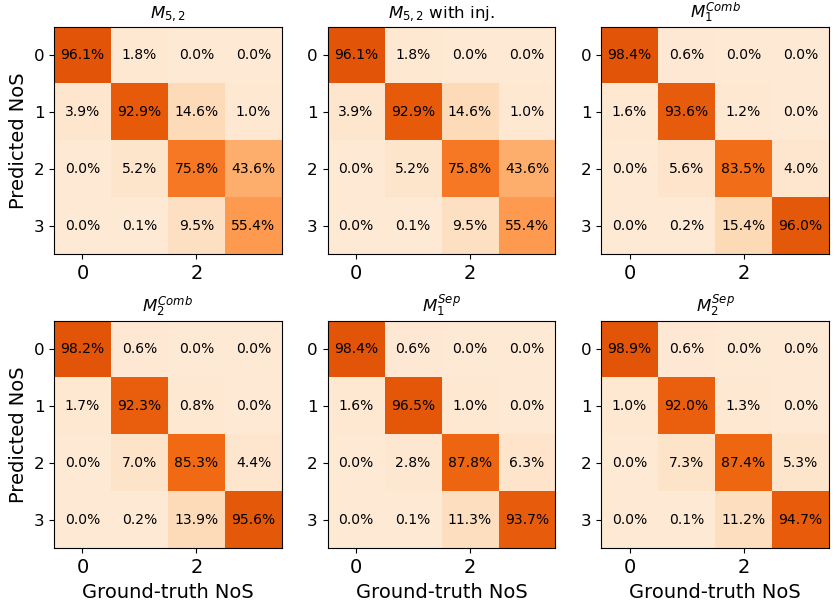
\includegraphics[width=1.\textwidth]{Images/chap8/hybrid_multitask_confusionMatrix_simulatedSrirs.png}
        \end{adjustbox}
    }\\
    \subfloat[Real SRIRs]{
        \begin{adjustbox}{width=1.1\textwidth,center}
            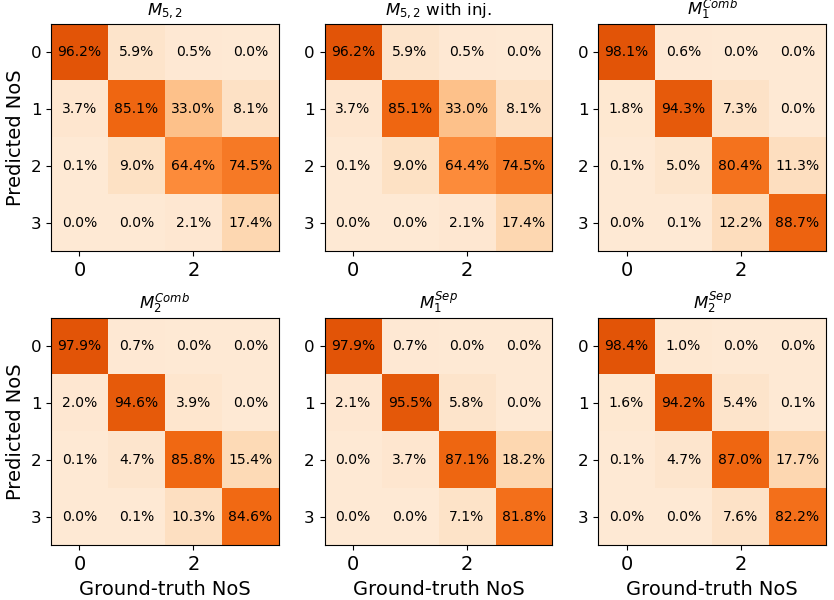
\includegraphics[width=1.\textwidth]{Images/chap8/hybrid_multitask_confusionMatrix_realSrirs.png}
        \end{adjustbox}
    }
    \captionof{figure}[Confusion matrices of the accuracy $A_{ij}$ for the multi-task neural networks and the model $M_{5,2}$ with and without injection]{Confusion matrices of the accuracy $A_{ij}$ for the multi-task neural networks and the model $M_{5,2}$  with and without NoS injection.}
    \label{fig:hybrid_multitask_confusionMatrices}
\end{figure}

\begin{figure}[t]
    \centering
    \subfloat[Simulated SRIRs]{
        \begin{adjustbox}{width=1.3\textwidth,center}
            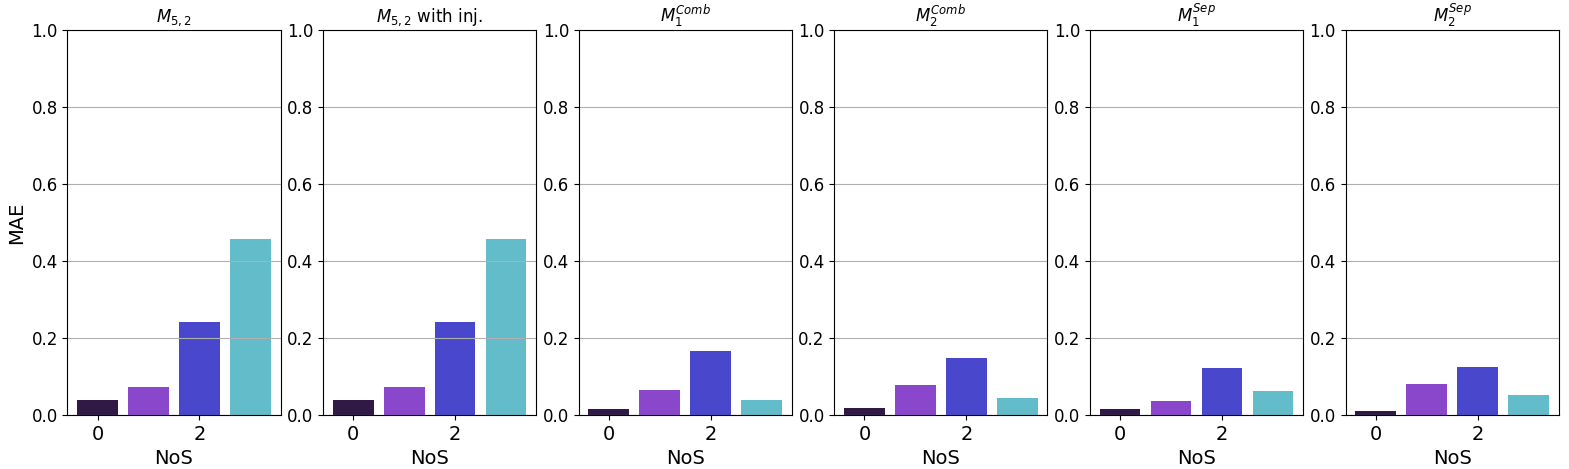
\includegraphics[width=1.\textwidth]{Images/chap8/hybrid_multitask_mae_simulatedSrirs.png}
        \end{adjustbox}
    }\\
    \subfloat[Real SRIRs]{
        \begin{adjustbox}{width=1.3\textwidth,center}
            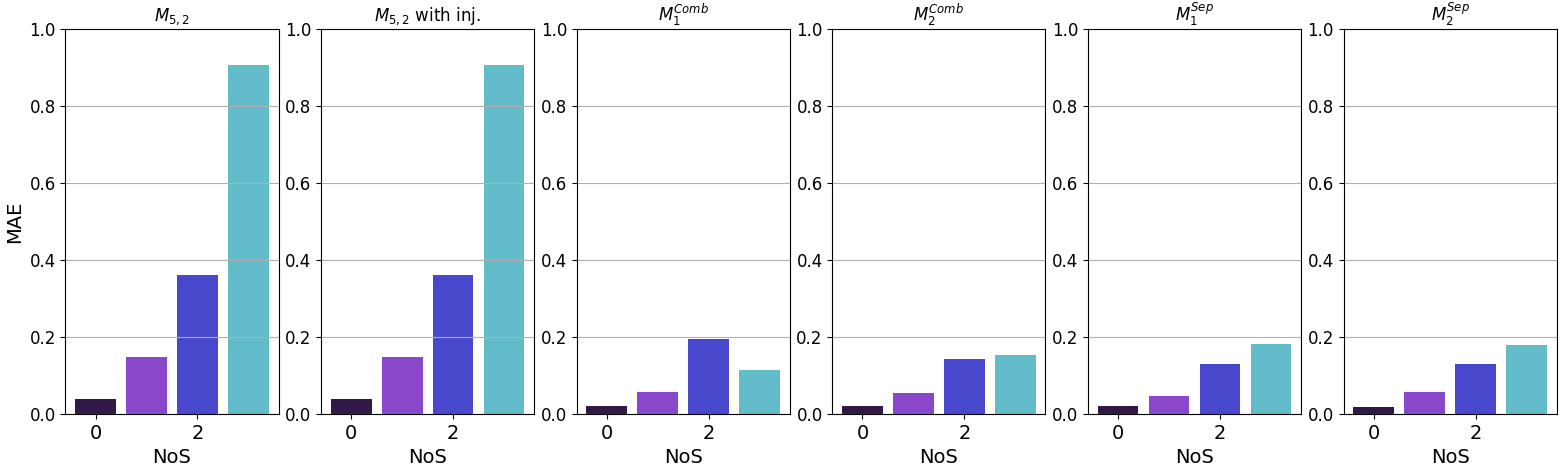
\includegraphics[width=1.\textwidth]{Images/chap8/hybrid_multitask_mae_realSrirs.png}
        \end{adjustbox}
    }
    \captionof{figure}[Mean absolute errors $M_i$ for the multi-task neural networks and the model $M_{5,2}$ with and without injection]{Mean absolute errors $M_i$ for the multi-task neural networks and the model $M_{5,2}$ with and without NoS injection.}
    \label{fig:hybrid_multitask_mae}
\end{figure}

\begin{figure}[t]
    \centering
    \begin{adjustbox}{width=1.2\textwidth,center}
        \subfloat[Simulated SRIRs]{
        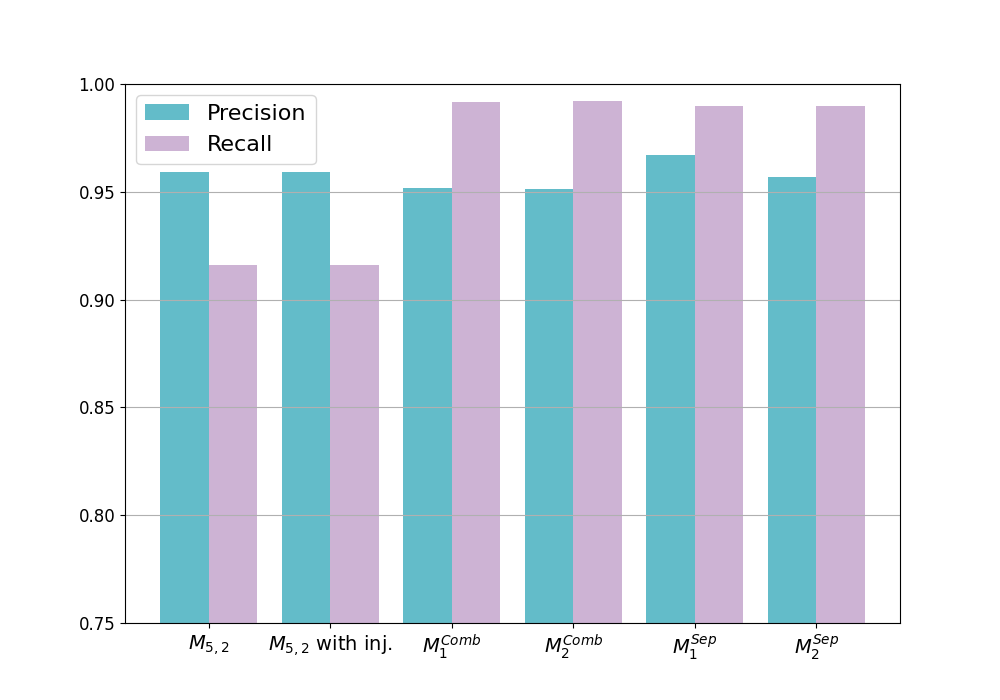
\includegraphics[width=.45\textwidth]{Images/chap8/hybrid_multitask_detection_simulatedSrirs.png}
        }
        \subfloat[Real SRIRs]{
            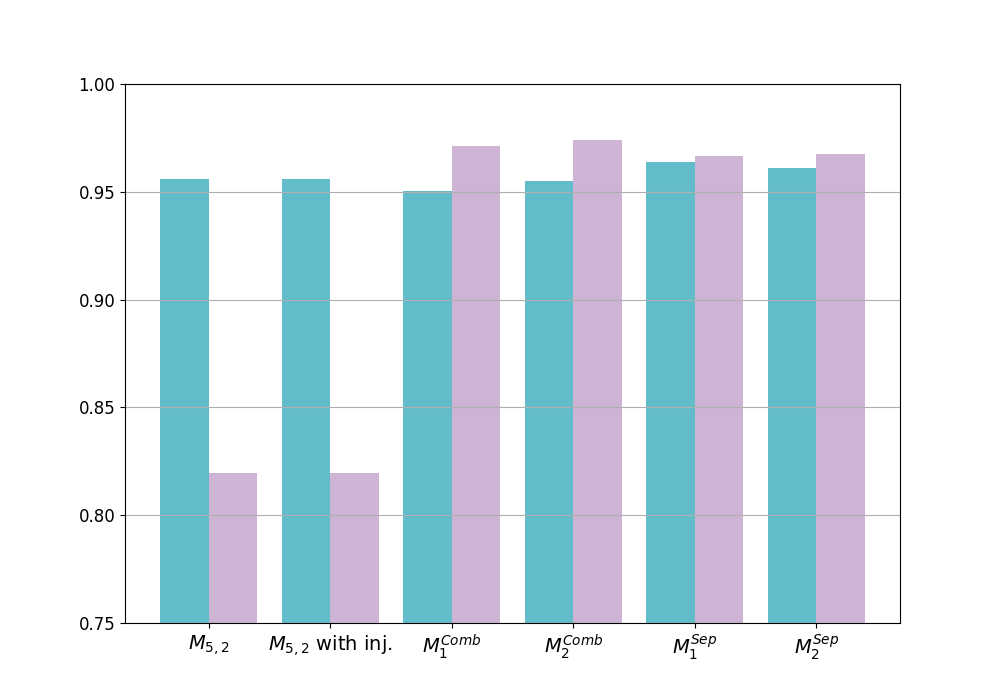
\includegraphics[width=.45\textwidth]{Images/chap8/hybrid_multitask_detection_realSrirs.png}
        }
    \end{adjustbox}
    \captionof{figure}[Detection precision and recall for the multi-task neural networks and the model $M_{5,2}$ with and without injection]{Detection precision and recall for the multi-task neural networks and the model $M_{5,2}$ with and without NoS injection.}
    \label{fig:hybrid_multitask_prediction}
\end{figure}



\clearpage
When looking at the confusion matrices in Fig.~\ref{fig:hybrid_multitask_confusionMatrices}, we can appreciate the robustness of the multi-task networks to count up to $3$ speakers, with more than $80$\% accuracy for all NoS on both simulated and real SRIRs. This approach also allows to greatly reduce the mean absolute error, as showed in Fig.~\ref{fig:hybrid_multitask_mae}, especially for $2$ and $3$ speakers, which does not exceed $0.2$ on both datasets. The detection metrics (see Fig.~\ref{fig:hybrid_multitask_prediction}) confirms the great performance of multi-task models over the baselines, with a source detection rate (recall) greater than $95$\% on real SRIRs in parallel with a relatively low false positive rate denoted by a precision of more than $95$\%, whereas for the counting-only network these metrics reached $96$\% and $82$\%, for precision and recall, respectively.

\begin{figure}[t]
    \centering
        \begin{adjustbox}{width=1.1\textwidth,center}
            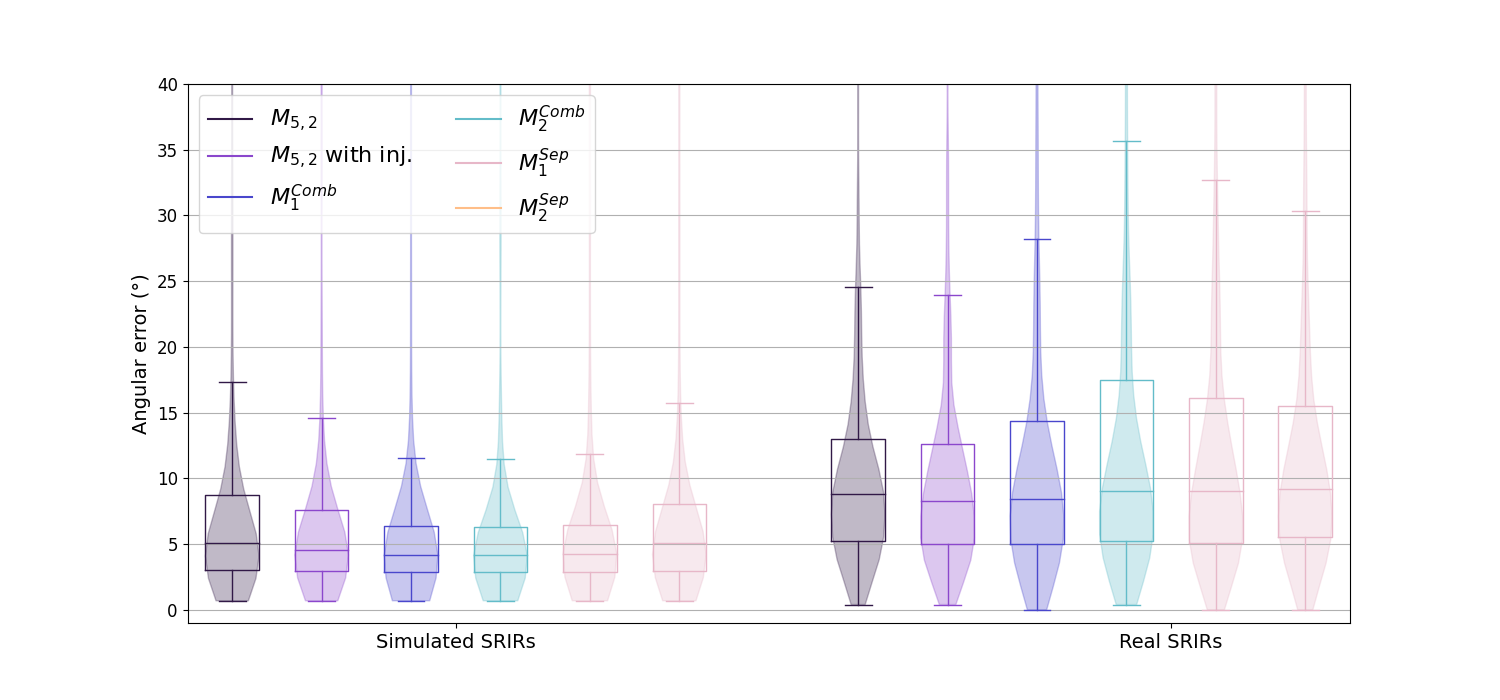
\includegraphics[width=.5\textwidth]{Images/chap8/hybrid_boxplots_multitask.png}
        \end{adjustbox}

    \captionof{figure}[Boxplots of the angular errors of the localization network for the multi-task neural networks and the model $M_{5,2}$ with and without injection]{Boxplots of the angular errors of the localization network for the multi-task neural networks and the model $M_{5,2}$ with and without NoS injection.}
    \label{fig:hybrid_boxplots_multitask}
\end{figure}

Regarding the localization results showed in Table~\ref{tab:hybrid_multitask_results} and Fig.~\ref{fig:hybrid_boxplots_multitask}, the multi-task networks are below the model $M_{5,2}$ with NoS injection on simulated SRIRs but are on par with the baseline $M_{5,2}$. On real SRIRs, we see that the multi-task networks lead to worse localization performance than the model $M_{5,2}$ with and without injection. However, recalling that the localization metrics are computed only for true positives, the results for the multi-task networks are in fact quite impressive given the very high detection recall. On simulated SRIRs, the multi-task networks are capable of detecting more speakers with a localization precision that remains at the level of the best baseline, although we can expect that some of the additional detected speakers are difficult to localize. Regarding the results on real SRIRs, they are below the baselines. Here, the effect of detecting more sources (and thus more sources that are difficult to localize and that lead to a quite high angular error) is probably more important, because of the larger difference in accuracy and recall with the baselines, compared to simulated SRIRs. For a more fair assessment, we can compare the localization results of the multi-task networks with those of the $M_{5,2}$ model when the latter uses an oracle counting system, leading to a comparable detection performance, as shown in Table~\ref{tab:hybrid_nosPrediction_localization}. We see that the localization accuracy ($<10$\textdegree) for the baseline $M_{5,2}$ is here $56.2$\% for real SRIRs, whereas it reaches $60.8$\% for the model $M^{Comb}_1$. Therefore, this seems to indicate that, for a similar counting/detection performance, the multi-task approach is performing better in localization compared with the baseline.

When comparing the different configurations of the multi-task neural network, we notice that for models $M^{Sep}$, adding a second feedforward layer tends to reduce the localization performance while not necessarily increasing the network counting and detection capability. For separate input features, the multi-task network with two feedforward layers performs $1.8$\% less in localization accuracy ($<10$\textdegree) than the same model with one feedforward layer, for simulated and real SRIRs, respectively. However the inverse observation can be made for models $M^{Comb}$, where $M^{Comb}_2$ is the one with the best localization results. Hence it is not straightforward to conclude about the interest of adding a second feedforward layer. Furthermore, it is not clear that separating the input features with a dedicating feature extraction module for each of them presents an advantage in such a multi-task system. The results on all multi-task networks are globally on par, whereas using two separate feature extraction modules leads to an important increase in the number of parameters (around $51$\% more). Finally when looking at the boxplots in Fig.~\ref{fig:hybrid_boxplots_multitask}, one can appreciate the fact that the multi-task networks detect more sources at the cost of a higher localization angular error variance, which seems to highlight the detection of sources more difficult to localize.

To conclude, the multi-task networks present quite impressive results in terms of counting and detection, compared to the use of a dedicated counting network as previously. The gain in counting performance is remarkable, especially on signals with real SRIRs. Regarding the localization performance, we can say that they almost reach the performance of the baseline model $M_{5,2}$ using an estimated NoS, which is quite impressive because of the high detection recall whereas the baseline's localization accuracy drastically drops when detecting more sources. It seems that the multi-task neural networks are capable of extracting high-level features that are relevant for both counting and localization. Feeding the input features separately in two different feature extraction modules or in combination in a single one has not provided convincing differences in performance. It seems that the overall improvement is due to the use of both input features and the network multi-task training. 

%-----------------------------------------------
%  CONCLUSION AND PERSPECTIVES
%-----------------------------------------------
\section{Conclusion and perspectives}

In this chapter, we have explored several ways of combining the counting and localization networks. In a first study, we assessed the benefit of using a separate counting network to estimate the NoS, before using this information to extract the right number of DoAs from a localization network output. We concluded that the speaker counting system is robust enough to be used in a practical use-case, as a replacement for the traditional NoS knowledge assumption that is made in research studies. Next, we investigated the interest of injecting the NoS information as an additional input feature to the localization network, with the idea that this can help to shape a more accurate DoA probability distribution output. By comparing the localization performance with and without NoS injection, as well as evaluating the robustness of using an estimated NoS instead of the ground-truth NoS, we demonstrated that this additional piece of information is valuable for the localization network, even if the performance gain is not considerable. Finally, we proposed to combine the counting and localization tasks into a single multi-task neural network, designed with two separate output branches for each task. We appropriately tuned the combination of the counting and localization loss functions with dedicated tests. Then, we showed the superiority of this multi-task approach over the use of two separate task-wise networks. We were able to largely improve the counting and detection performance, while the localization performance were globally remaining at a level very close to the baseline. This is a quite satisfactory result, considering the high detection accuracy and the fact that sources that are difficult to detect (not detected by the baseline) may also be difficult to localize. The experiments dealing with the order of the combination module and the feature extraction module to combine the different input features have not been conclusive, since the results obtained with the two solutions were on par.

The research work presented in this chapter leads to several questions and perspectives. First, the proposal of injecting the NoS, based on the idea that a robust estimate NoS could help the localization network for a better output distributions, has not led to an important increase in localization accuracy, especially on real-world signals. A first idea would be to use the NoS probability distribution, estimated by the counting network, instead of a one-hot encoded vector which drops possibly precious information. A general perspective to address the issue of real-world data performance lies in the deep learning research effort to adapt neural network trained with simulated data on real-world data. In the specific context of this work, we believe that there might be a better manner to help the localization network with this precious NoS information. As we pointed out in other chapters, analyzing in depth how the neural network uses the NoS information could give some insights. Another intriguing interesting aspect gravitates around the proposed (variants of the) multi-task neural network, especially regarding the reason why the counting performance has been largely improved with this system compared to the baseline. Analyzing where does this improvement come from --which we did not have time to conduct-- would help us understand what network aspect is crucial for source counting. Is it the feature extraction module? (we recall the proposed perspective at the end of Chapter~\ref{chap:counting}), the combined input features? the benefit of jointly learning counting and localization? Also, it would be great to comprehend the way the multi-task network uses the same extracted feature --and the contents of this feature-- for two tied but distinct tasks.
